% Options for packages loaded elsewhere
\PassOptionsToPackage{unicode}{hyperref}
\PassOptionsToPackage{hyphens}{url}
\PassOptionsToPackage{dvipsnames,svgnames,x11names}{xcolor}
%
\documentclass[
  letterpaper,
  DIV=11,
  numbers=noendperiod]{scrreprt}

\usepackage{amsmath,amssymb}
\usepackage{lmodern}
\usepackage{iftex}
\ifPDFTeX
  \usepackage[T1]{fontenc}
  \usepackage[utf8]{inputenc}
  \usepackage{textcomp} % provide euro and other symbols
\else % if luatex or xetex
  \usepackage{unicode-math}
  \defaultfontfeatures{Scale=MatchLowercase}
  \defaultfontfeatures[\rmfamily]{Ligatures=TeX,Scale=1}
\fi
% Use upquote if available, for straight quotes in verbatim environments
\IfFileExists{upquote.sty}{\usepackage{upquote}}{}
\IfFileExists{microtype.sty}{% use microtype if available
  \usepackage[]{microtype}
  \UseMicrotypeSet[protrusion]{basicmath} % disable protrusion for tt fonts
}{}
\makeatletter
\@ifundefined{KOMAClassName}{% if non-KOMA class
  \IfFileExists{parskip.sty}{%
    \usepackage{parskip}
  }{% else
    \setlength{\parindent}{0pt}
    \setlength{\parskip}{6pt plus 2pt minus 1pt}}
}{% if KOMA class
  \KOMAoptions{parskip=half}}
\makeatother
\usepackage{xcolor}
\setlength{\emergencystretch}{3em} % prevent overfull lines
\setcounter{secnumdepth}{5}
% Make \paragraph and \subparagraph free-standing
\ifx\paragraph\undefined\else
  \let\oldparagraph\paragraph
  \renewcommand{\paragraph}[1]{\oldparagraph{#1}\mbox{}}
\fi
\ifx\subparagraph\undefined\else
  \let\oldsubparagraph\subparagraph
  \renewcommand{\subparagraph}[1]{\oldsubparagraph{#1}\mbox{}}
\fi


\providecommand{\tightlist}{%
  \setlength{\itemsep}{0pt}\setlength{\parskip}{0pt}}\usepackage{longtable,booktabs,array}
\usepackage{calc} % for calculating minipage widths
% Correct order of tables after \paragraph or \subparagraph
\usepackage{etoolbox}
\makeatletter
\patchcmd\longtable{\par}{\if@noskipsec\mbox{}\fi\par}{}{}
\makeatother
% Allow footnotes in longtable head/foot
\IfFileExists{footnotehyper.sty}{\usepackage{footnotehyper}}{\usepackage{footnote}}
\makesavenoteenv{longtable}
\usepackage{graphicx}
\makeatletter
\def\maxwidth{\ifdim\Gin@nat@width>\linewidth\linewidth\else\Gin@nat@width\fi}
\def\maxheight{\ifdim\Gin@nat@height>\textheight\textheight\else\Gin@nat@height\fi}
\makeatother
% Scale images if necessary, so that they will not overflow the page
% margins by default, and it is still possible to overwrite the defaults
% using explicit options in \includegraphics[width, height, ...]{}
\setkeys{Gin}{width=\maxwidth,height=\maxheight,keepaspectratio}
% Set default figure placement to htbp
\makeatletter
\def\fps@figure{htbp}
\makeatother

\KOMAoption{captions}{tableheading}
\makeatletter
\makeatother
\makeatletter
\@ifpackageloaded{bookmark}{}{\usepackage{bookmark}}
\makeatother
\makeatletter
\@ifpackageloaded{caption}{}{\usepackage{caption}}
\AtBeginDocument{%
\ifdefined\contentsname
  \renewcommand*\contentsname{Table of contents}
\else
  \newcommand\contentsname{Table of contents}
\fi
\ifdefined\listfigurename
  \renewcommand*\listfigurename{List of Figures}
\else
  \newcommand\listfigurename{List of Figures}
\fi
\ifdefined\listtablename
  \renewcommand*\listtablename{List of Tables}
\else
  \newcommand\listtablename{List of Tables}
\fi
\ifdefined\figurename
  \renewcommand*\figurename{Figure}
\else
  \newcommand\figurename{Figure}
\fi
\ifdefined\tablename
  \renewcommand*\tablename{Table}
\else
  \newcommand\tablename{Table}
\fi
}
\@ifpackageloaded{float}{}{\usepackage{float}}
\floatstyle{ruled}
\@ifundefined{c@chapter}{\newfloat{codelisting}{h}{lop}}{\newfloat{codelisting}{h}{lop}[chapter]}
\floatname{codelisting}{Listing}
\newcommand*\listoflistings{\listof{codelisting}{List of Listings}}
\makeatother
\makeatletter
\@ifpackageloaded{caption}{}{\usepackage{caption}}
\@ifpackageloaded{subcaption}{}{\usepackage{subcaption}}
\makeatother
\makeatletter
\@ifpackageloaded{tcolorbox}{}{\usepackage[many]{tcolorbox}}
\makeatother
\makeatletter
\@ifundefined{shadecolor}{\definecolor{shadecolor}{rgb}{.97, .97, .97}}
\makeatother
\makeatletter
\makeatother
\ifLuaTeX
  \usepackage{selnolig}  % disable illegal ligatures
\fi
\IfFileExists{bookmark.sty}{\usepackage{bookmark}}{\usepackage{hyperref}}
\IfFileExists{xurl.sty}{\usepackage{xurl}}{} % add URL line breaks if available
\urlstyle{same} % disable monospaced font for URLs
\hypersetup{
  pdftitle={Sistema de reporte de avances},
  pdfauthor={Samuel Calderon},
  colorlinks=true,
  linkcolor={blue},
  filecolor={Maroon},
  citecolor={Blue},
  urlcolor={Blue},
  pdfcreator={LaTeX via pandoc}}

\title{Sistema de reporte de avances}
\author{Samuel Calderon}
\date{}

\begin{document}
\maketitle
\ifdefined\Shaded\renewenvironment{Shaded}{\begin{tcolorbox}[borderline west={3pt}{0pt}{shadecolor}, breakable, sharp corners, interior hidden, enhanced, boxrule=0pt, frame hidden]}{\end{tcolorbox}}\fi

\renewcommand*\contentsname{Table of contents}
{
\hypersetup{linkcolor=}
\setcounter{tocdepth}{2}
\tableofcontents
}
\bookmarksetup{startatroot}

\hypertarget{prefacio}{%
\chapter*{Prefacio}\label{prefacio}}
\addcontentsline{toc}{chapter}{Prefacio}

\markboth{Prefacio}{Prefacio}

La Dirección de Control de Drogas y Cultivos Ilegales del Ministerio del
Interior ha implementado un sistema informático para la gestión de la
información de los avances en las tareas cotidianas y automatización de
la generación de reportes.

Este documento contiene las instrucciones para el uso del sistema
informático.

Si estás viendo este manual desde una computadora, el menú izquierdo
permite acceder a diferentes capítulos del manual. Desde un teléfono,
este menú se encuentra en la parte superior.

\bookmarksetup{startatroot}

\hypertarget{manual-de-usuario}{%
\chapter{Manual de usuario}\label{manual-de-usuario}}

\hypertarget{creaciuxf3n-de-nueva-tarea}{%
\section{Creación de nueva tarea}\label{creaciuxf3n-de-nueva-tarea}}

La creación de una nueva tarea se hace desde el menú de la columna
``Pendiente''. Se debe hacer click en el botón \texttt{...} y escoger el
item ``Nueva tarea''.

\begin{figure}

{\centering 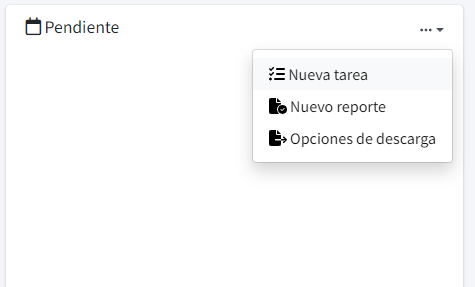
\includegraphics[width=4.16667in,height=\textheight]{./img/manual-user/pending-menu.png}

}

\end{figure}

Nos aparecerá una ventana en la que podemos llenar información de la
tarea. A continuación se explica el contenido de cada campo.

\hypertarget{tuxedtulo-de-tarea}{%
\subsection{Título de tarea}\label{tuxedtulo-de-tarea}}

El título de tarea es la información principal a visualizar. Brinda una
idea general de la tarea que se busca completar. Al redactar el título
debe buscarse mantenerlo corto pero lo suficientemente claro para no
confundirlo con otras tareas.

Puede tener como máximo 250 caracteres.

\begin{figure}

{\centering 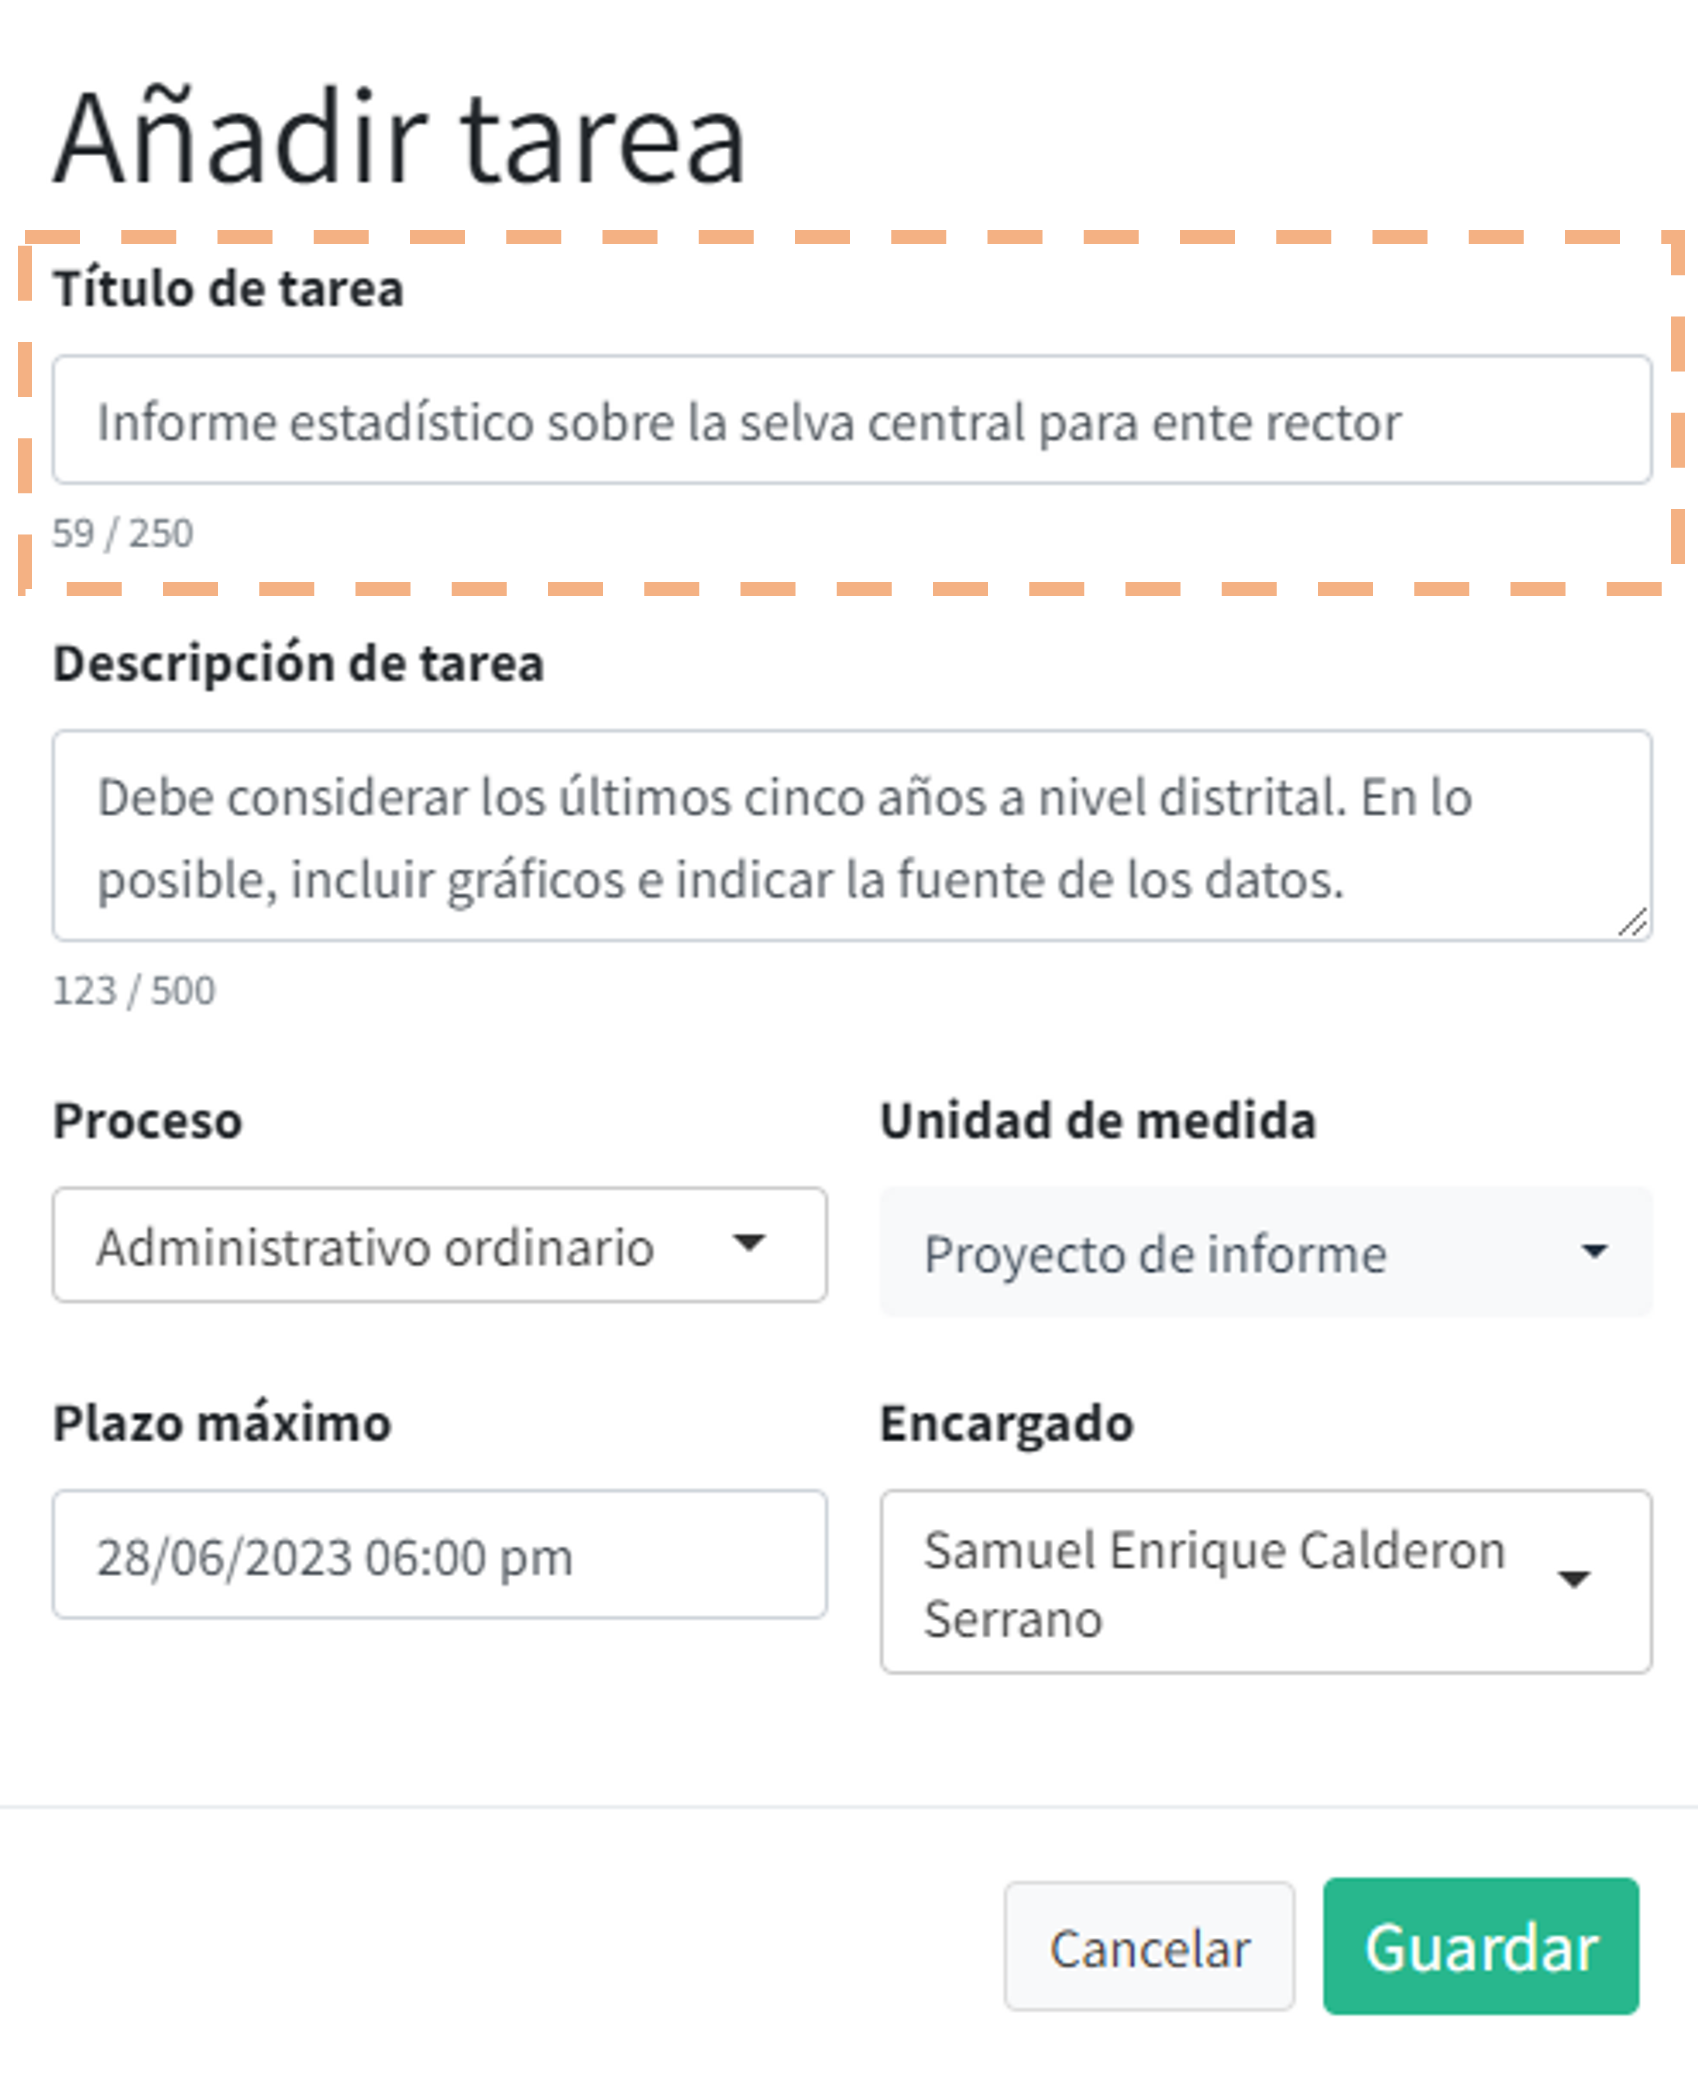
\includegraphics[width=4.16667in,height=\textheight]{./img/manual-user/new-task-title.png}

}

\end{figure}

\hypertarget{descripciuxf3n-de-tarea}{%
\subsection{Descripción de tarea}\label{descripciuxf3n-de-tarea}}

La descripción de tarea brinda mayor detalle acerca del contenido,
metodología o fuentes a utilizar para completar la tarea. Dentro de este
campo es posible explayarse para brindar mayor especificidad a la tarea.

Puede tener como máximo 500 caracteres.

\begin{figure}

{\centering 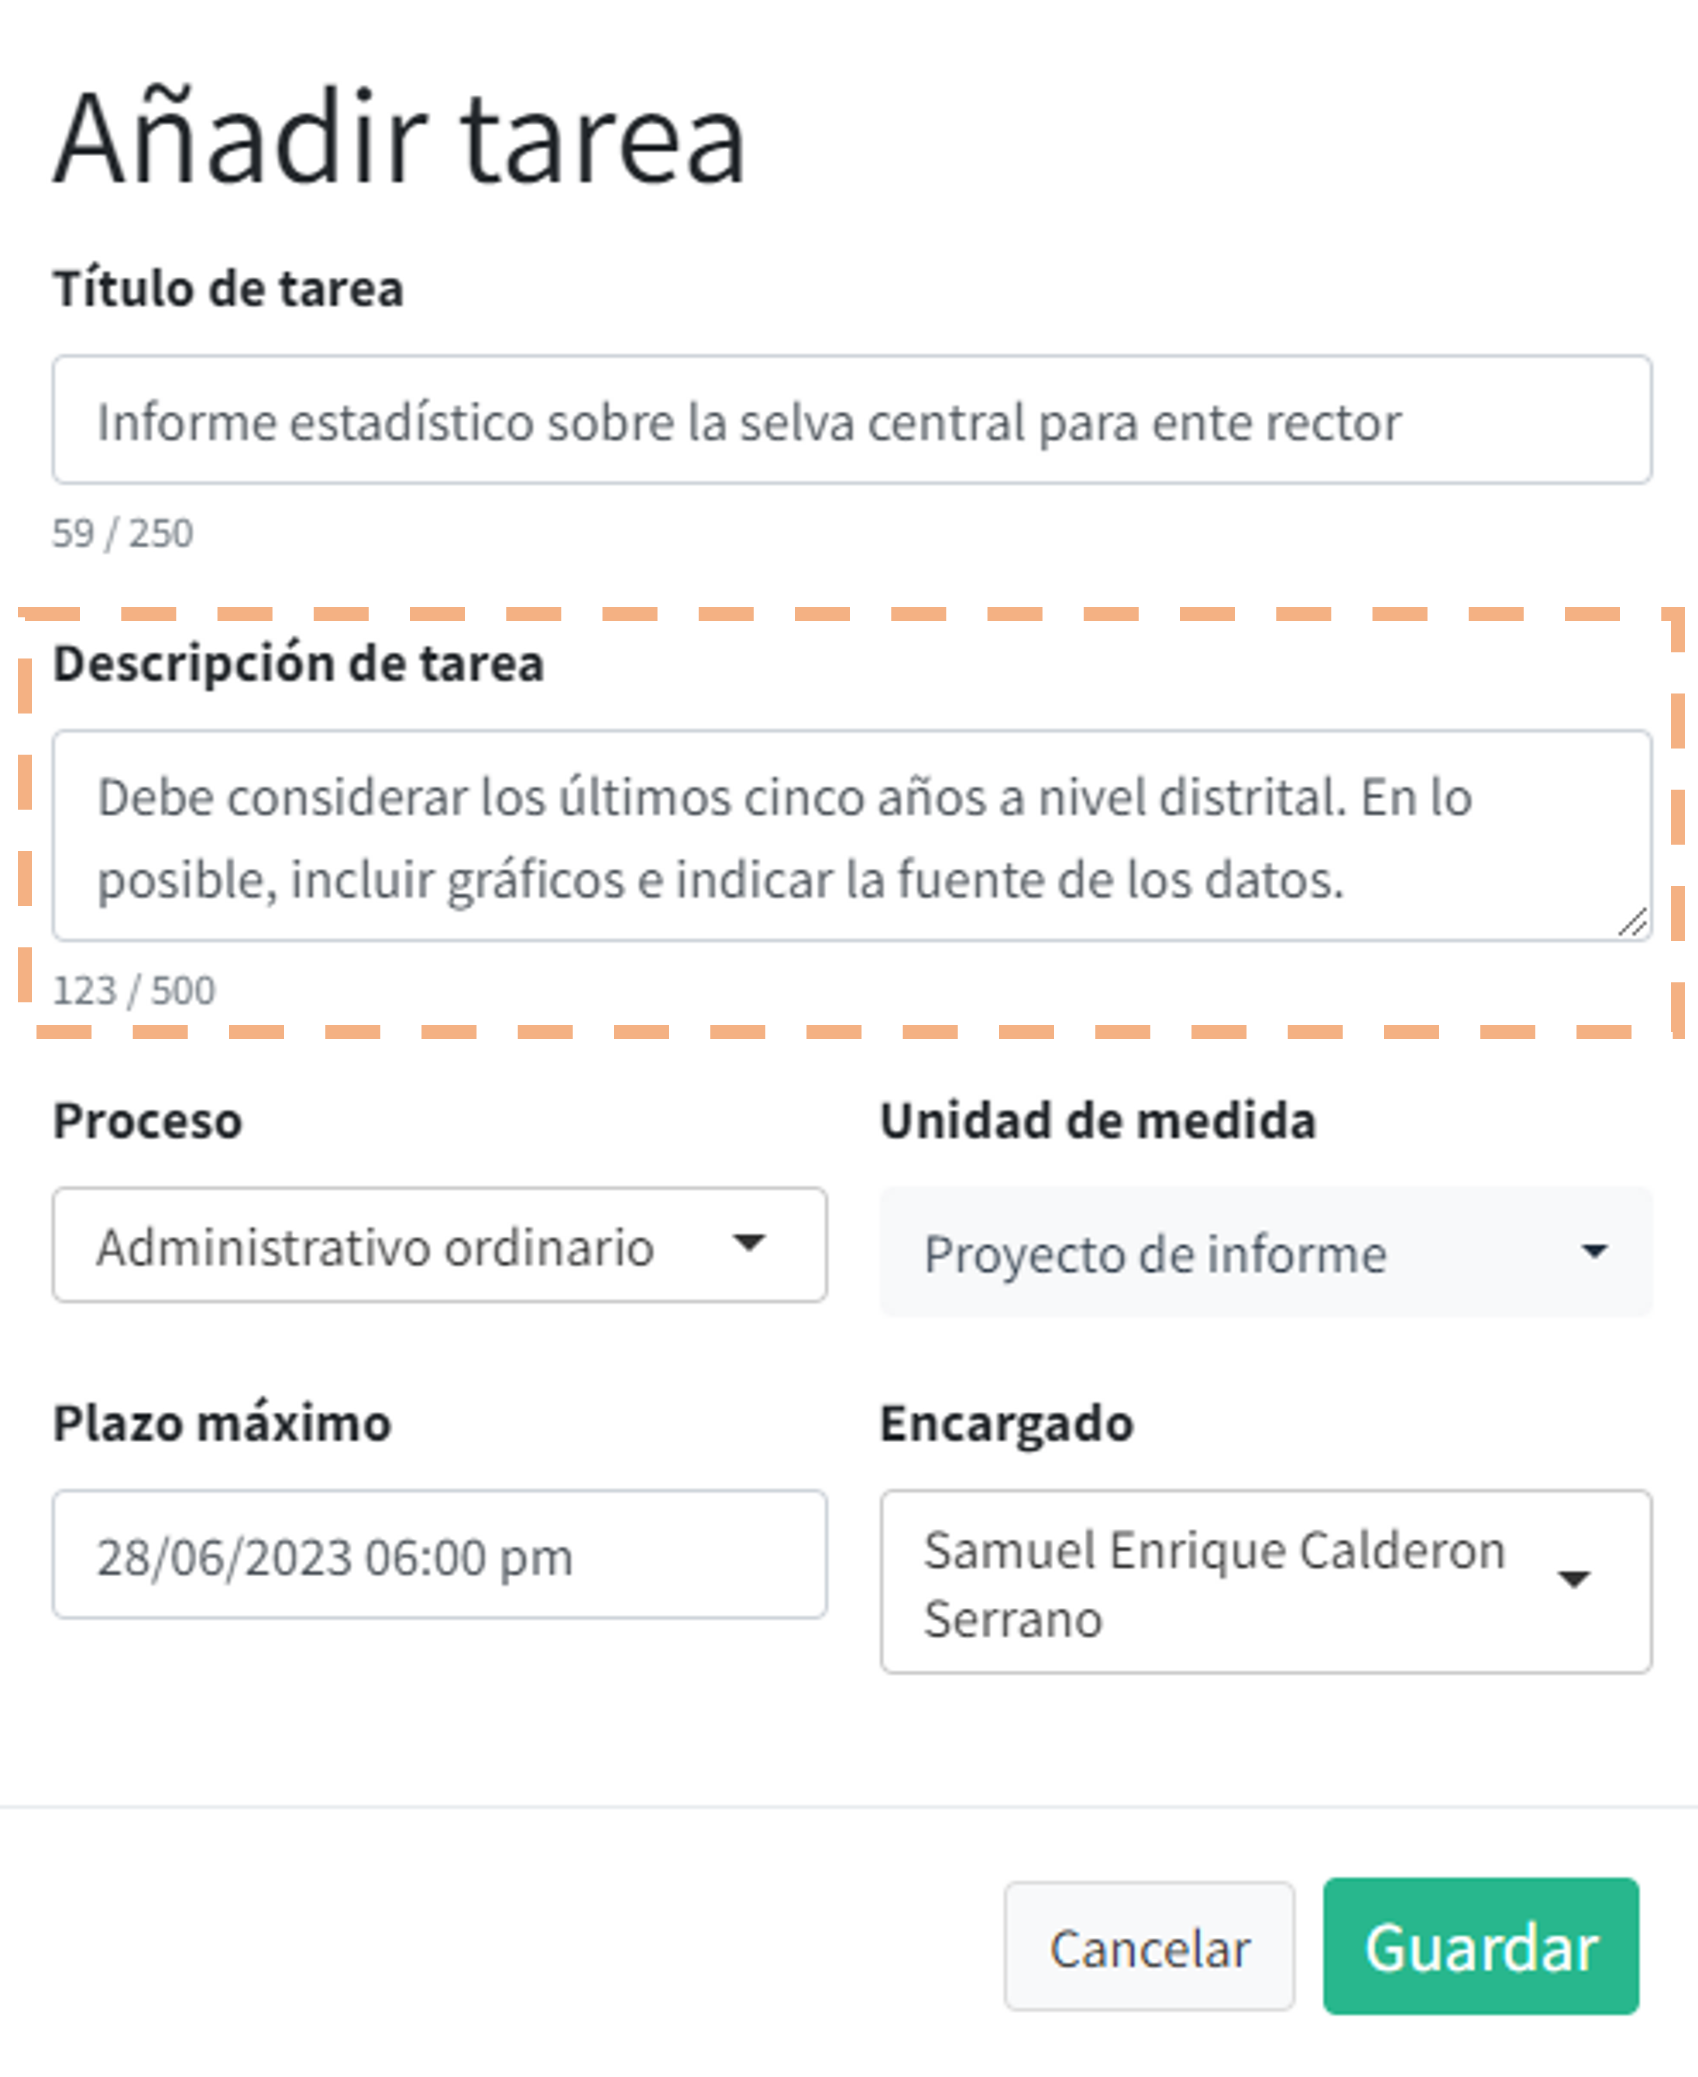
\includegraphics[width=4.16667in,height=\textheight]{./img/manual-user/new-task-description.png}

}

\end{figure}

\hypertarget{proceso}{%
\section{Proceso}\label{proceso}}

Es un conjunto de actividades llevadas a cabo para alcanzar algún fin en
particular. En el contexto de la gestión de tareas, sirve para agrupar
distintas unidades de medida que aportan en un fin común o una tarea
mayor, vinculada a algún producto de la unidad funcional.

\begin{figure}

{\centering 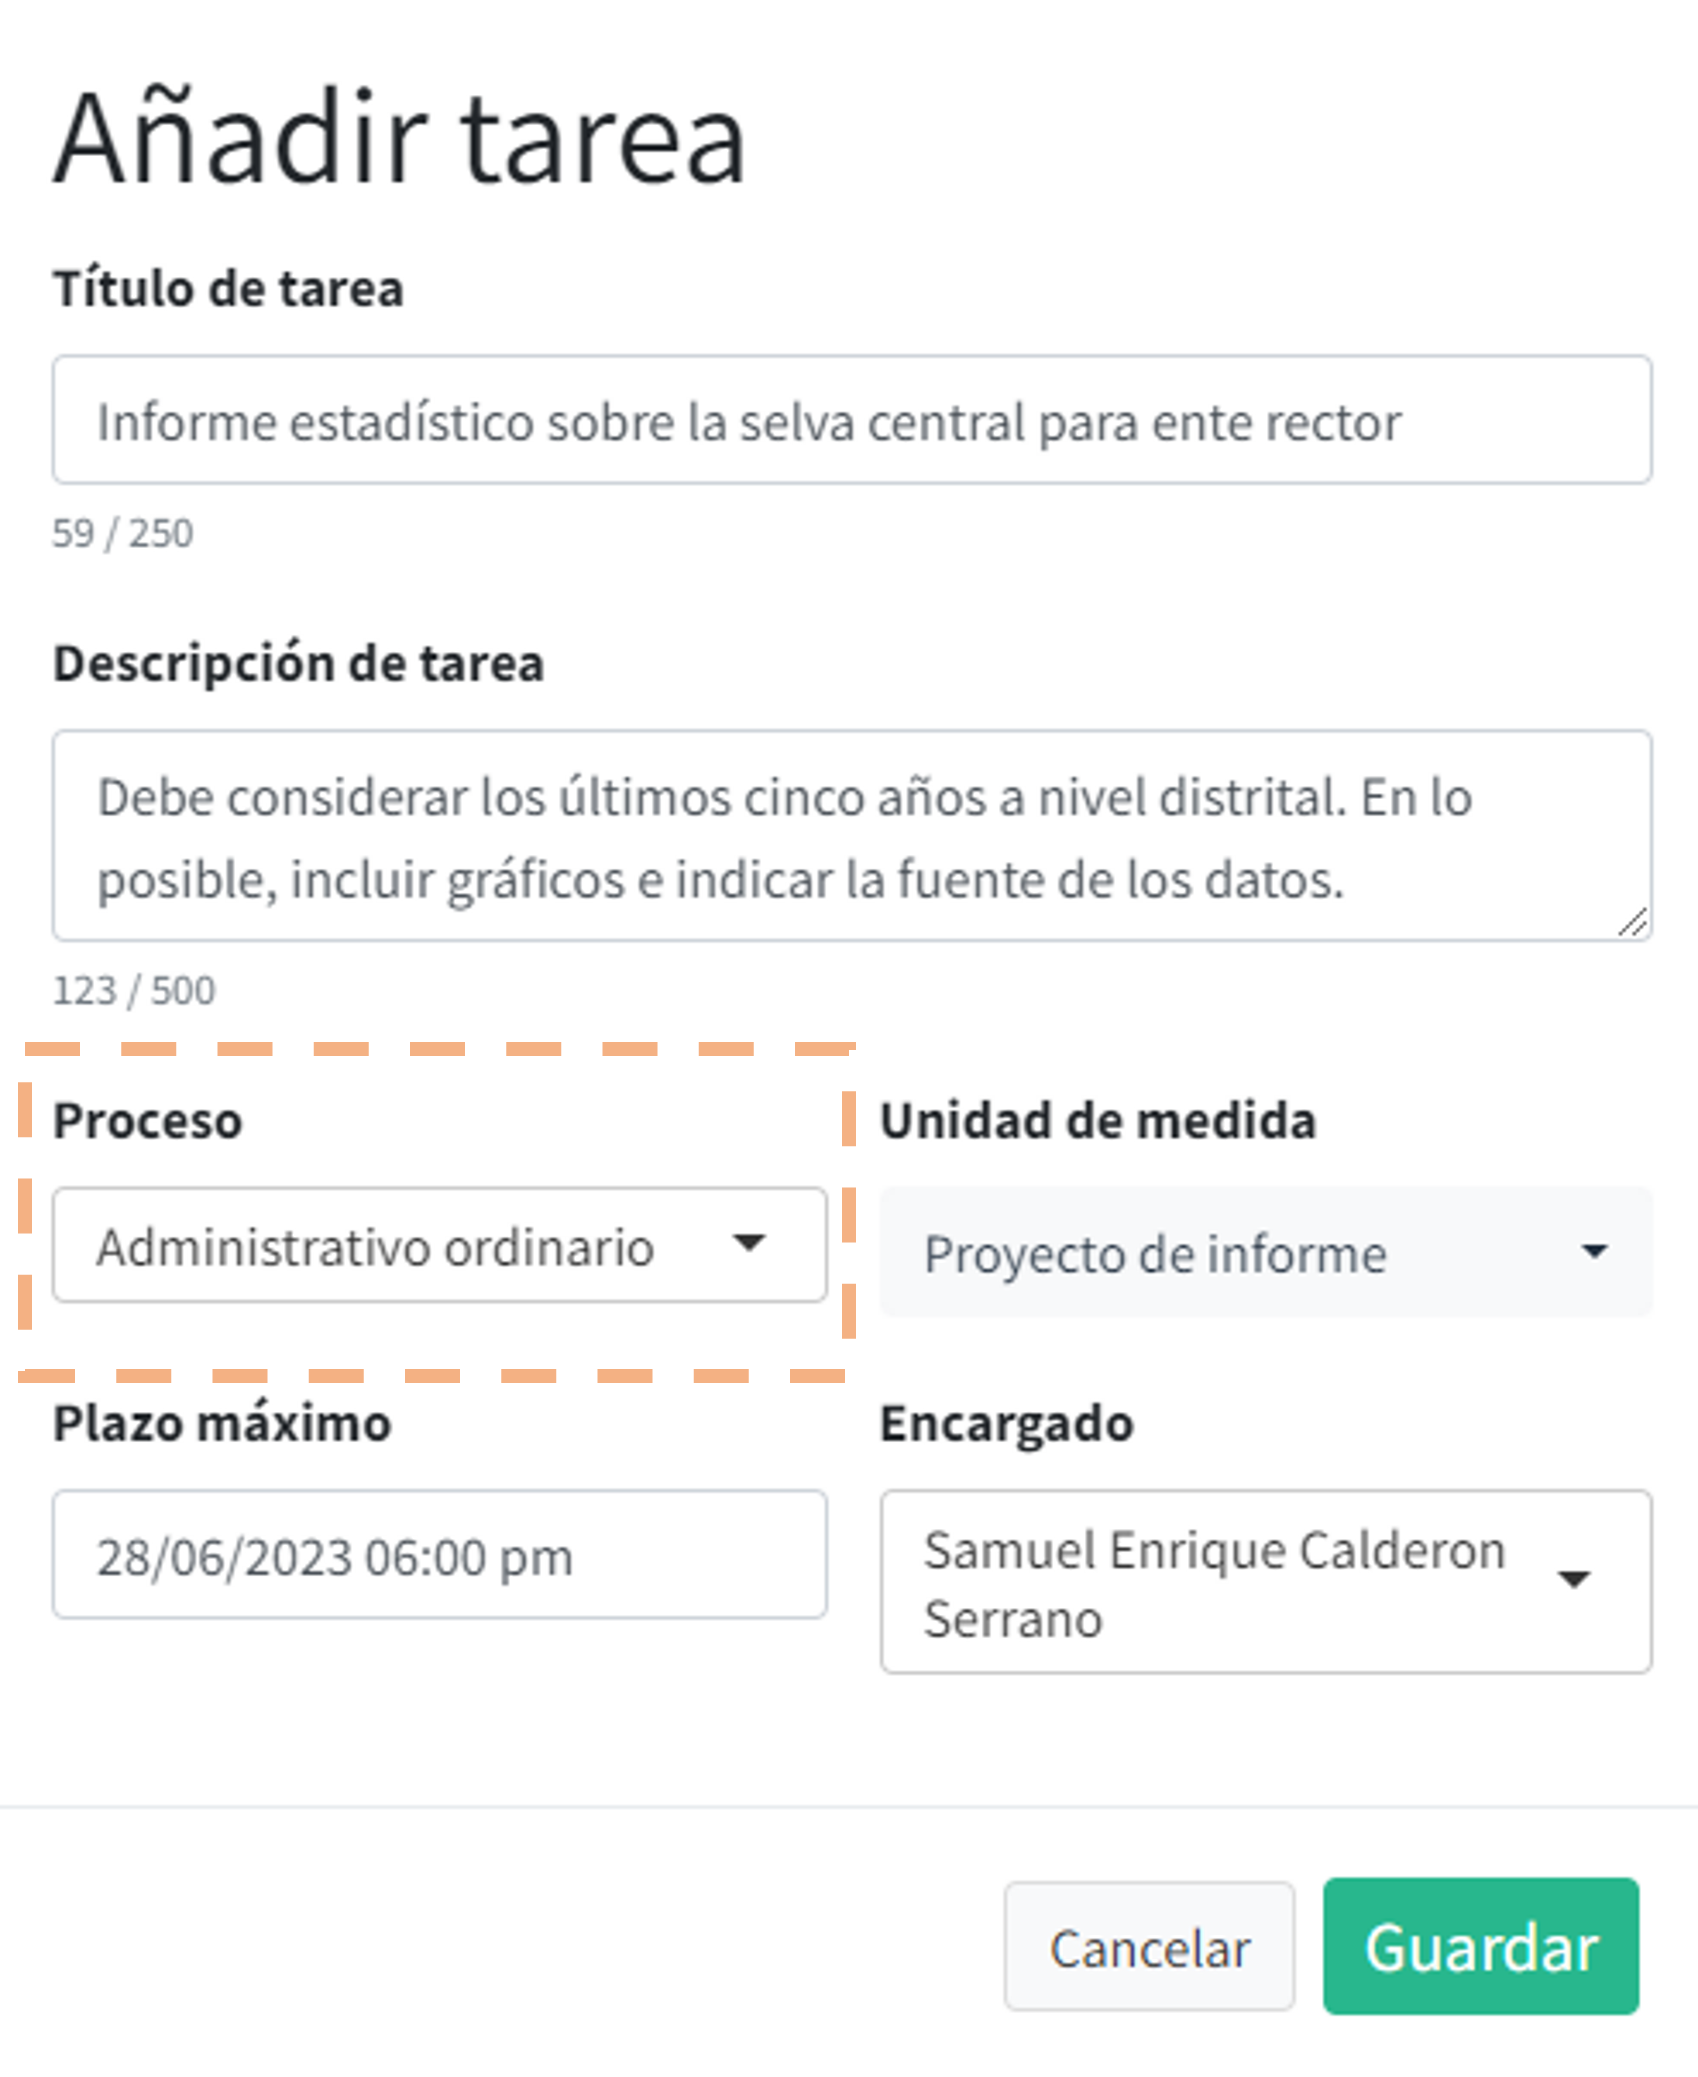
\includegraphics[width=4.16667in,height=\textheight]{./img/manual-user/new-task-process.png}

}

\end{figure}

\hypertarget{sec-unidad-de-medida}{%
\subsection{Unidad de medida}\label{sec-unidad-de-medida}}

Es el producto o evidencia medible de que la tarea se ha completado.
Cuando la tarea se marque como terminada, aumentará una unidad en el
contador de producción para la unidad de medida escogida.

Por defecto, se espera que las tareas produzcan un informe. Sin embargo,
las opciones de unidad de medida disponibles deben ser personalizadas de
acuerdo al trabajo que se realiza en el equipo.

\begin{figure}

{\centering 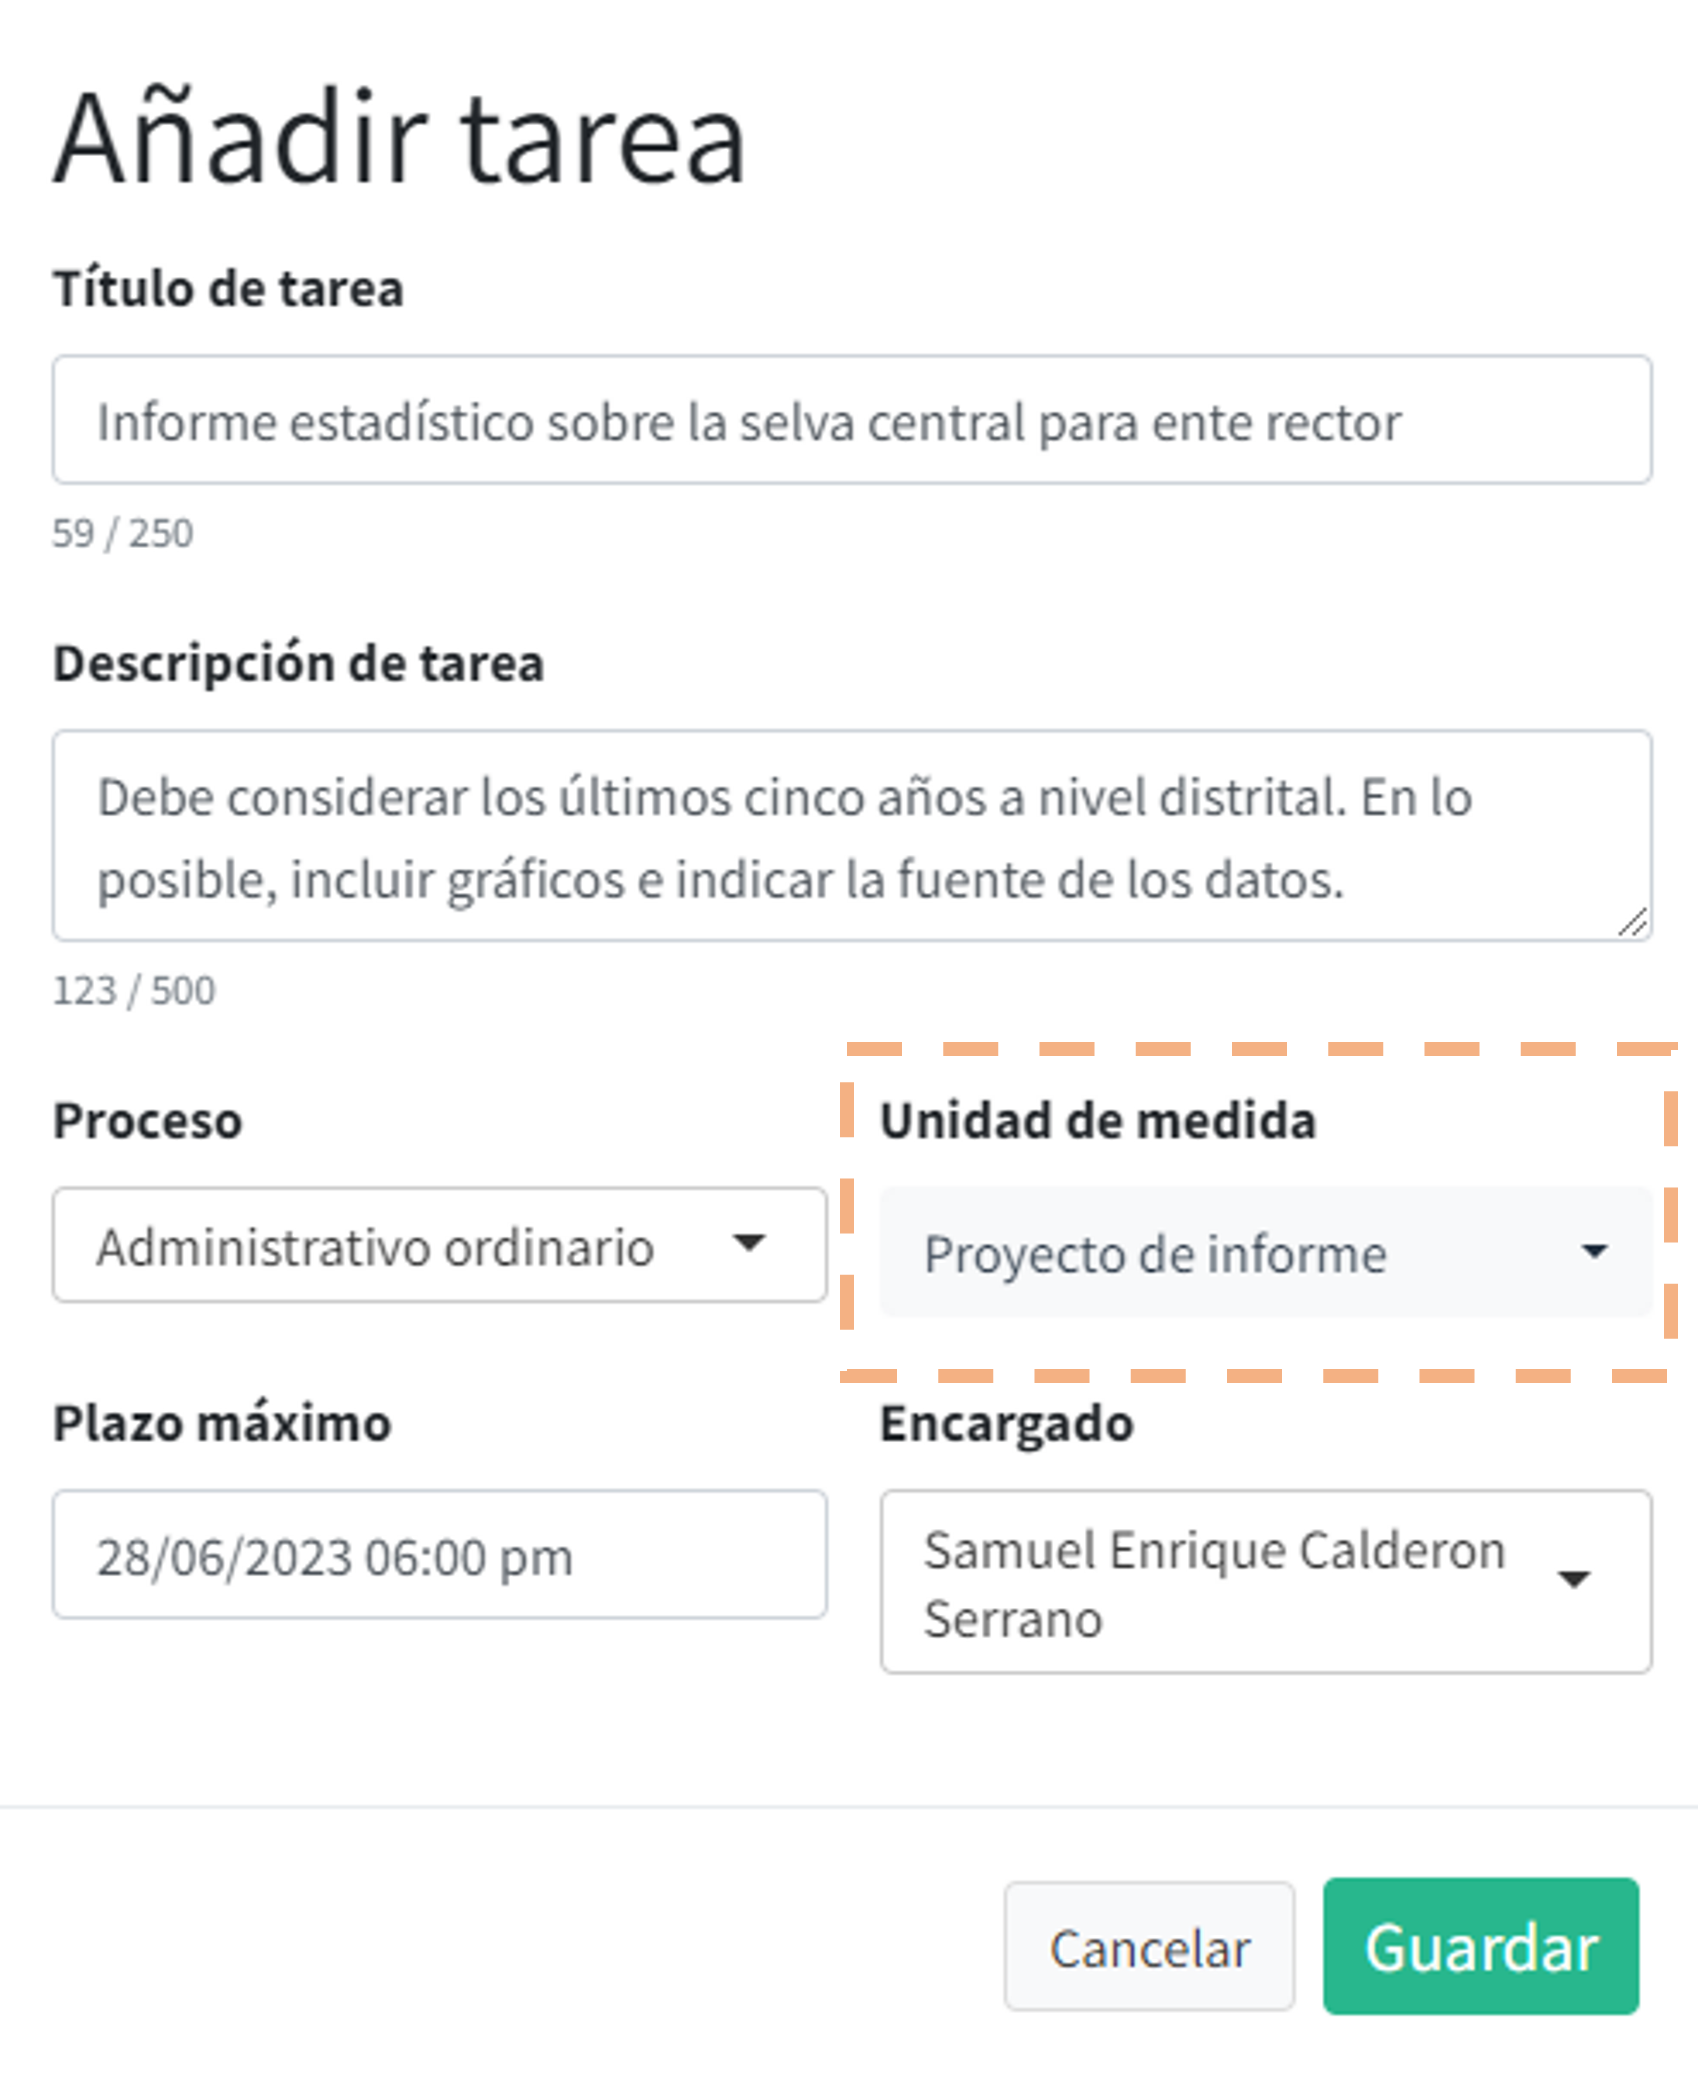
\includegraphics[width=4.16667in,height=\textheight]{./img/manual-user/new-task-unit.png}

}

\end{figure}

\hypertarget{plazo-muxe1ximo}{%
\subsection{Plazo máximo}\label{plazo-muxe1ximo}}

Establece una fecha y hora límites para el cumplimiento de la tarea.
Respecto a la hora límite, es posible escogerla en el rango de las 8:00
hasta las 18:45. Por defecto, el sistema establece el día siguiente a la
fecha de creación de la tarea.

\begin{figure}

{\centering 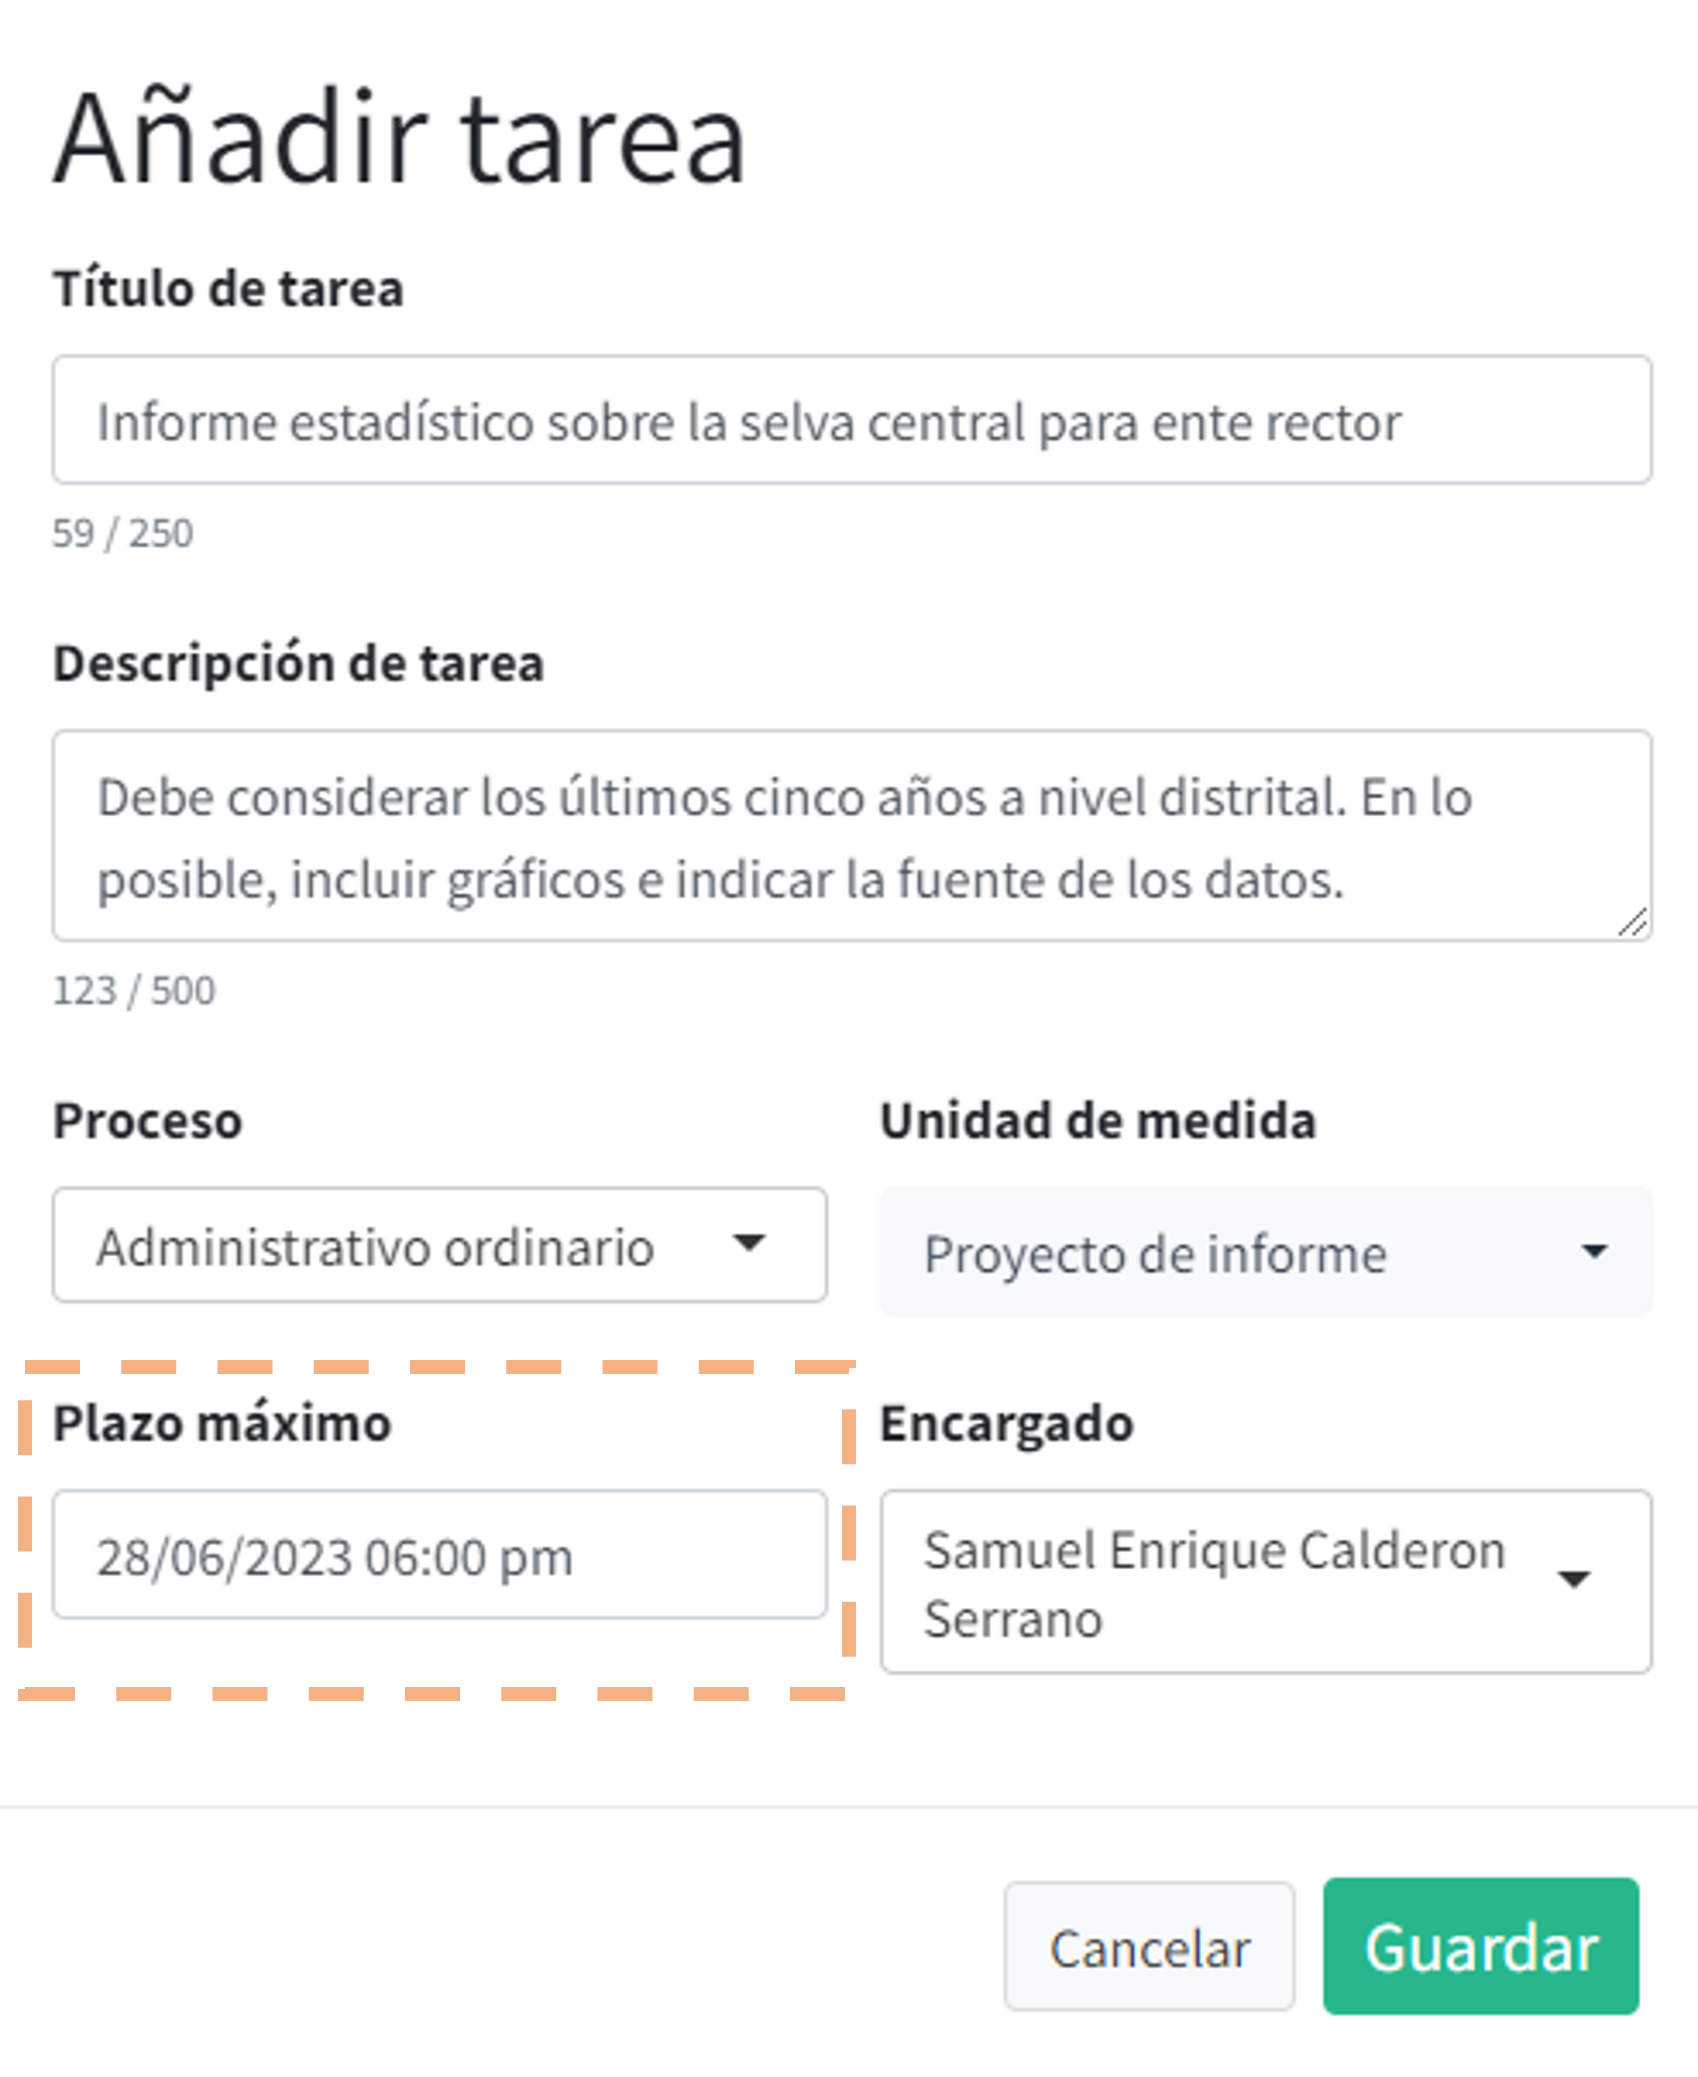
\includegraphics[width=4.16667in,height=\textheight]{./img/manual-user/new-task-timedue.png}

}

\end{figure}

\hypertarget{encargado}{%
\subsection{Encargado}\label{encargado}}

Indica el nombre de la persona responsable del cumplimiento de la tarea.
Un usuario básico solo puede escoger su nombre, pero un usuario
responsable de equipo puede asignarle tareas a otras personas dentro de
su equipo.

\begin{figure}

{\centering 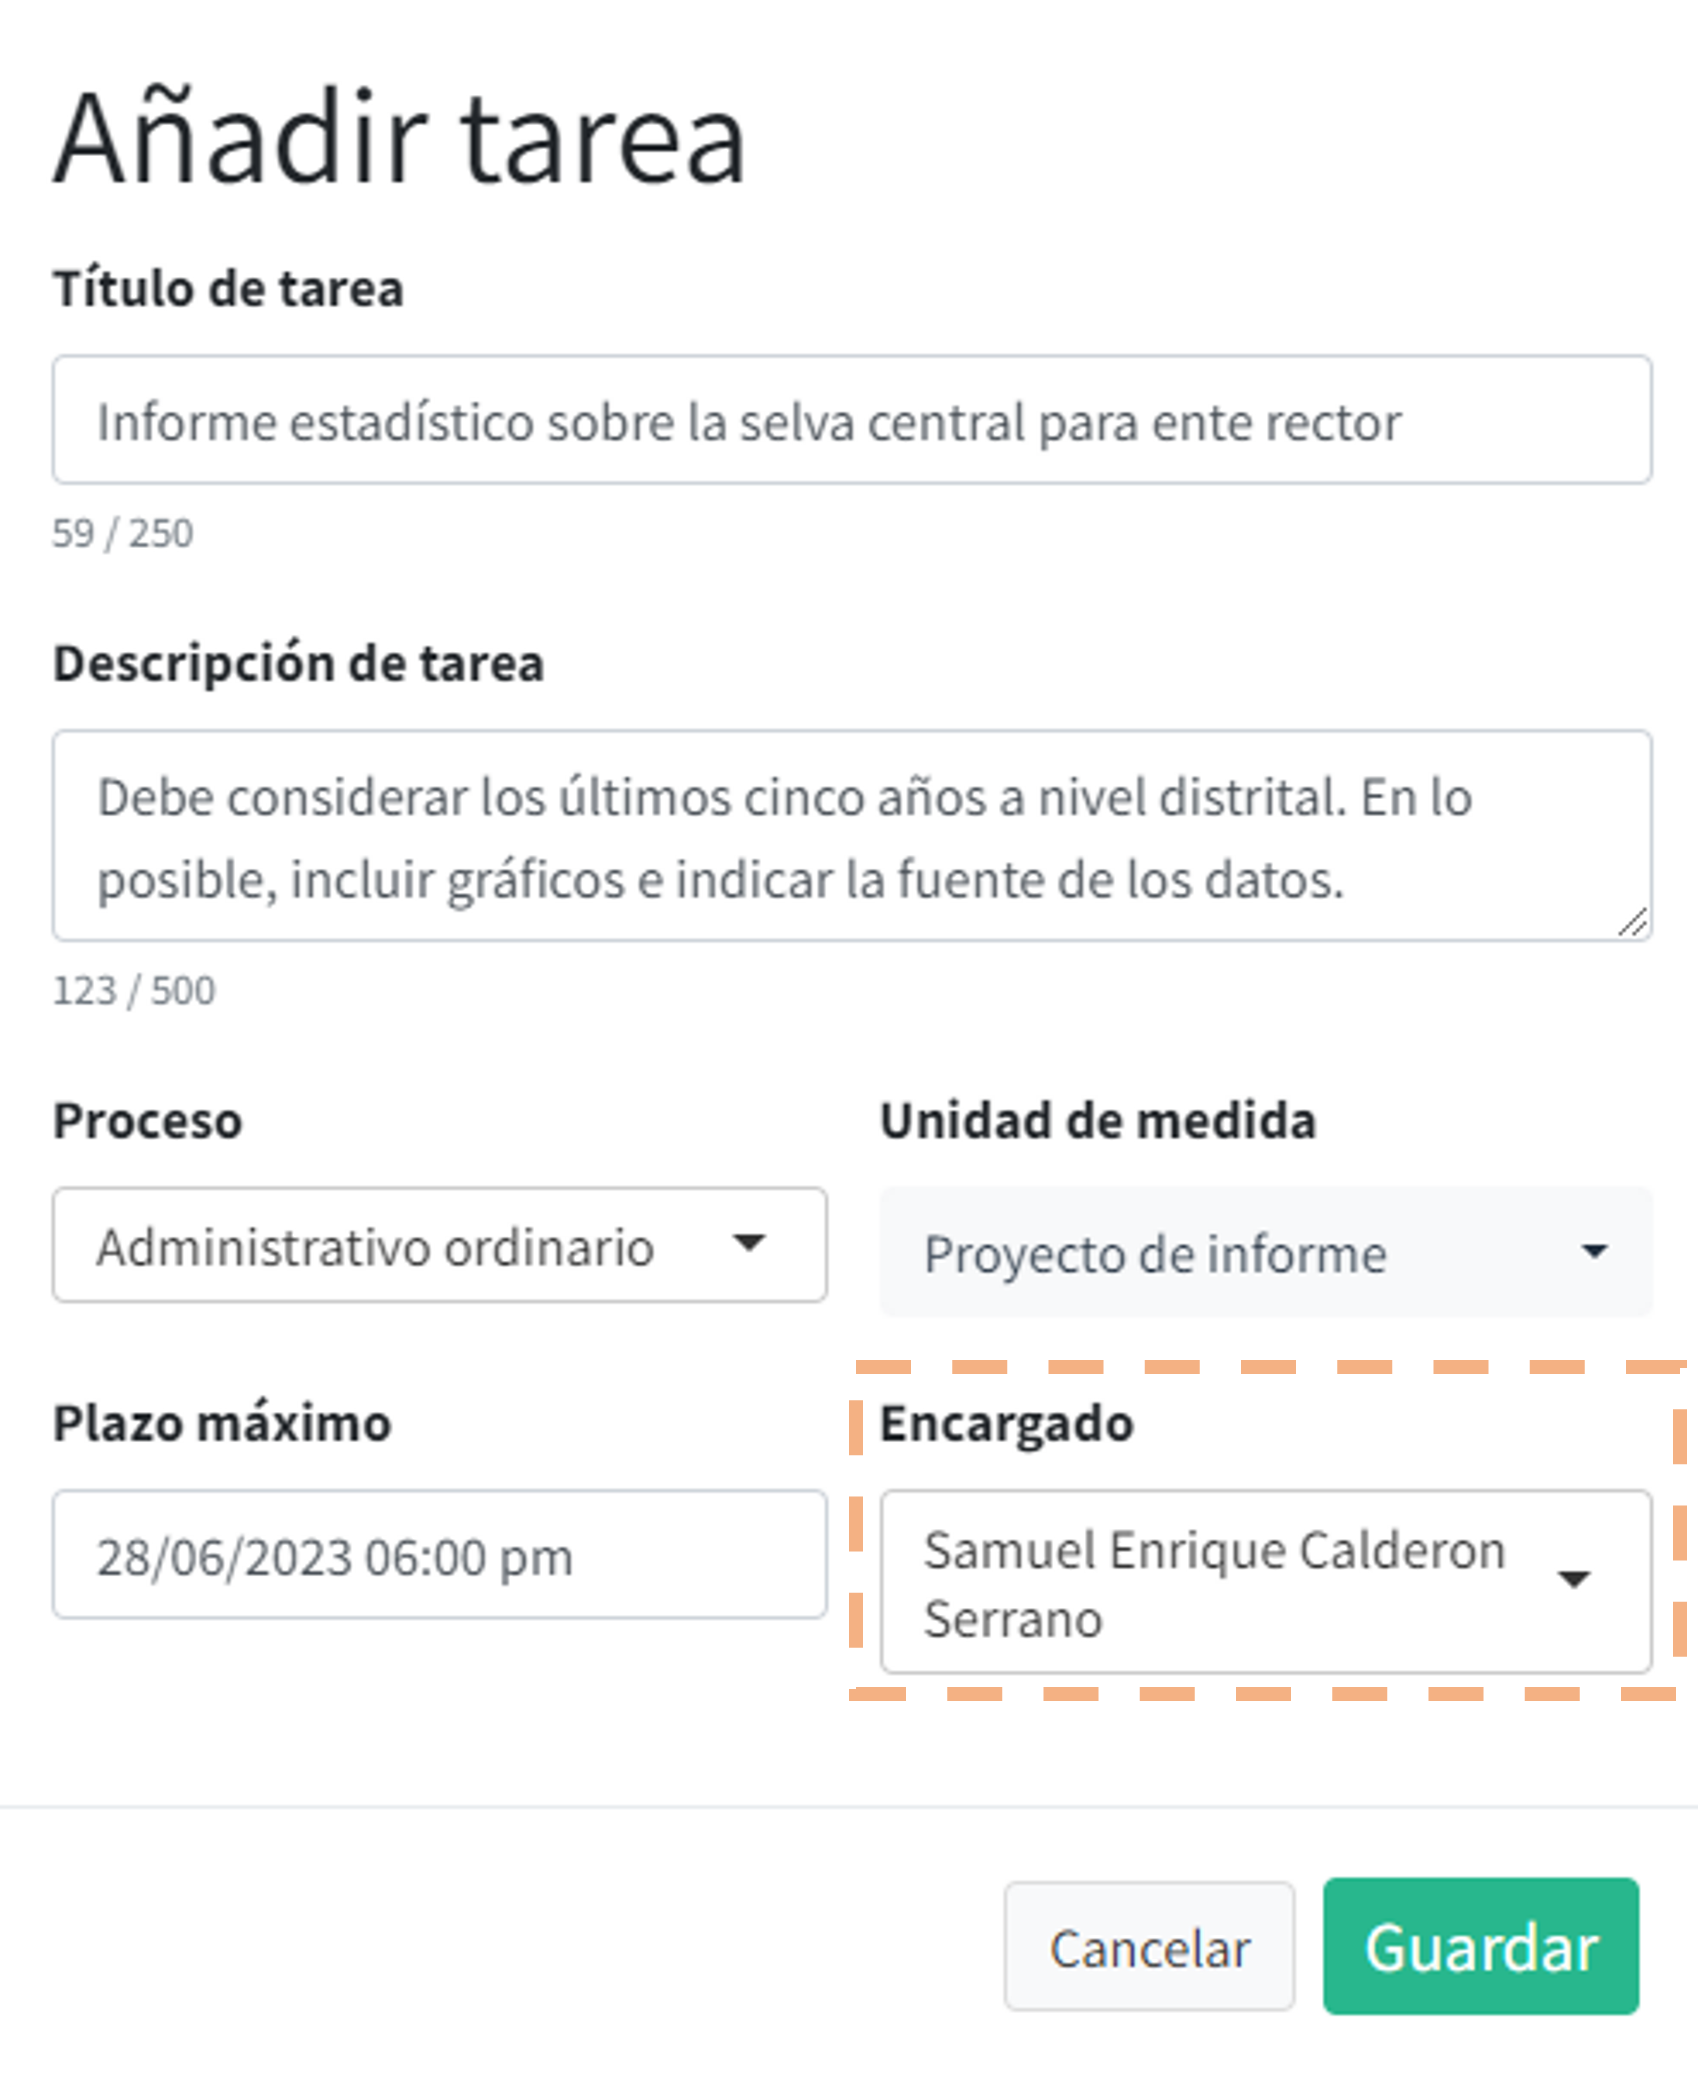
\includegraphics[width=4.16667in,height=\textheight]{./img/manual-user/new-task-assignee.png}

}

\end{figure}

\hypertarget{gestiuxf3n-de-progreso-de-tareas}{%
\section{Gestión de progreso de
tareas}\label{gestiuxf3n-de-progreso-de-tareas}}

Cada tarea asignada es convertida en una tarjeta dentro de la
plataforma.

\hypertarget{tarjeta-de-tarea}{%
\subsection{Tarjeta de tarea}\label{tarjeta-de-tarea}}

Al iniciar la aplicación, todas las tarjetas inician en un estado
cerrado, en la que solo es posible ver el título de la tarea y su fecha
límite. Todas las tareas recién creadas aparecen en la columna de
``Pendientes''.

\begin{figure}

{\centering 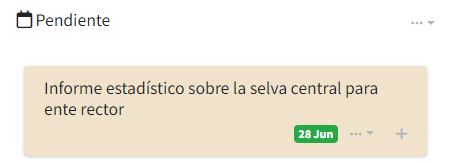
\includegraphics[width=4.16667in,height=\textheight]{./img/manual-user/task-closed.png}

}

\end{figure}

El color de la etiqueta en la que aparece la fecha límite variará según
qué tan cerca se esté de ella al momento de ver la tarjeta:

\begin{itemize}
\item
  Verde: Hasta el día previo de la fecha límite
\item
  Amarillo: El día de fecha límite
\item
  Rojo: Desde un día después de la fecha límite
\end{itemize}

De esta manera se puede hacer un seguimiento rápido a las tareas que
sean más urgentes.

Al hacer click en el botón \texttt{+} la tarjeta mostrará información
extra de la tarea.

\begin{figure}

{\centering 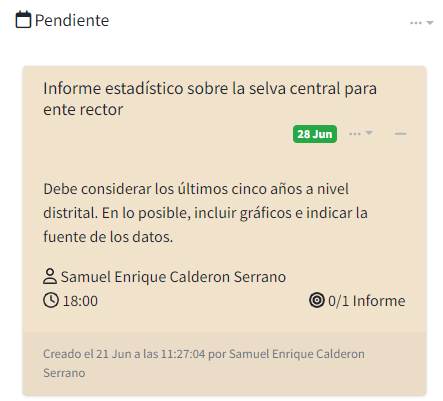
\includegraphics[width=4.16667in,height=\textheight]{./img/manual-user/task-open.png}

}

\end{figure}

La información extra incluye la descripción, el nombre de la persona
responsable, la hora límite y la unidad de medida establecida.La parte
inferior de la tarjeta muestra la fecha y hora de creación, así como la
persona que asignó la tarea.

Al presionar sobre el símbolo de menú (\texttt{…}) se obtienen opciones
de acción para la gestión de la tarea.

\begin{figure}

{\centering 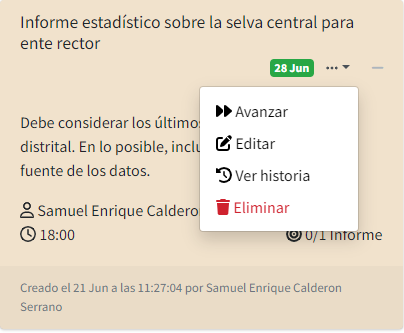
\includegraphics[width=4.16667in,height=\textheight]{./img/manual-user/task-menu.png}

}

\end{figure}

\hypertarget{avanzar}{%
\subsection{Avanzar}\label{avanzar}}

Permite avanzar en el \protect\hyperlink{sec-ciclo-de-vida}{ciclo de
vida} de la tarea. Inicialmente la tarea tiene un estado ``Pendiente'',
pero con esta opción podemos registrar algún tipo de progreso. Darle
click en ``Avanzar'' abre una ventana que modifica el estado de la
tarea.

\begin{figure}

{\centering 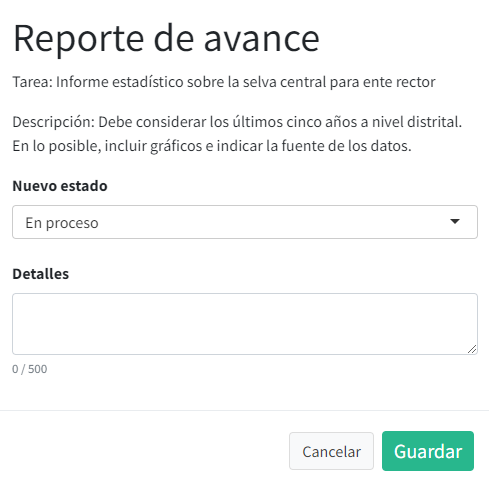
\includegraphics[width=4.16667in,height=\textheight]{./img/manual-user/task-progress.png}

}

\end{figure}

Las opciones para elegir el nuevo estado de la tarea dependerán del
estado actual de la tarea. Por ejemplo, desde ``Pendiente'' es posible
indicar que la tarea está ``En proceso'' o ``En revisión''.

Por último, el campo ``Detalles'' permite brindar información extra
sobre el progreso reportado, como señalar coordinaciones, revisiones o
cumplimientos parciales. Si está resultando difícil completar los plazos
establecidos, pueden indicarse razones en esta celda.

Una vez guardado el progreso, la tarjeta de tarea aparecerá en la
columna correspondiente al nuevo estado.

\hypertarget{editar}{%
\subsection{Editar}\label{editar}}

Permite cambiar el título o descripción de la tarea. Utilizarlo en caso
de que la redacción de alguno de ellos ya no resulte satisfactoria o sea
necesario actualizar la fecha límite de entrega.

\begin{figure}

{\centering 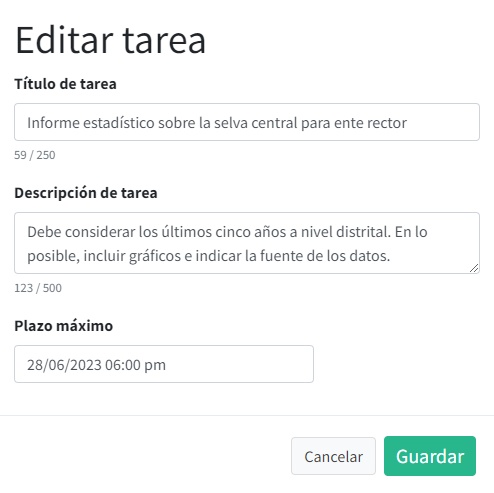
\includegraphics[width=4.16667in,height=\textheight]{./img/manual-user/task-edit.png}

}

\end{figure}

Cada edición genera una entrada en el historial de la tarea.

\hypertarget{ver-historia}{%
\subsection{Ver historia}\label{ver-historia}}

Permite ver todos los reportes de progreso reportados en esta tarea o
sus ediciones. Indica la fecha y hora de reporte, persona que reportó,
estado de la tarea y el detalle provisto.

\begin{figure}

{\centering 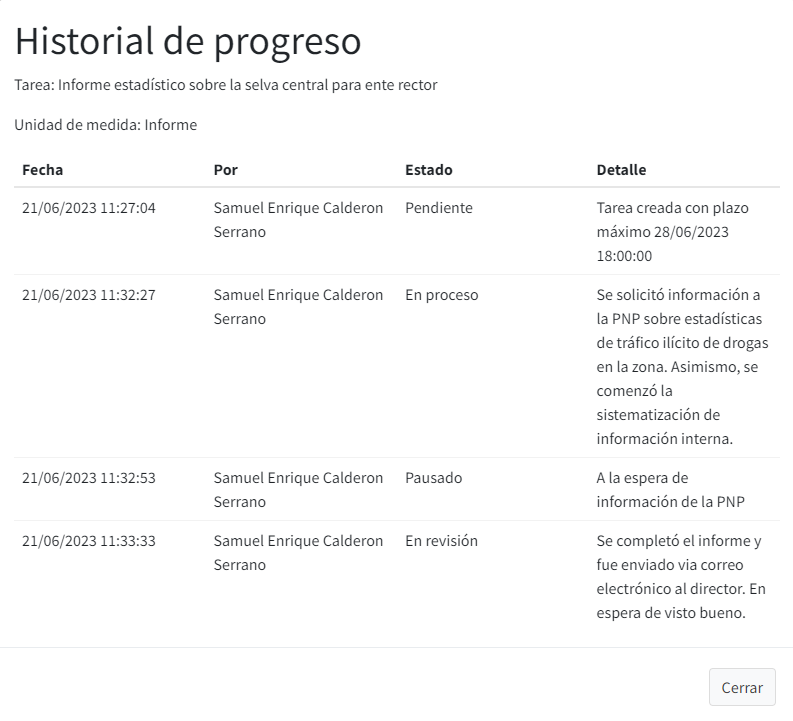
\includegraphics[width=6.25in,height=\textheight]{./img/manual-user/task-history.png}

}

\end{figure}

\hypertarget{eliminar}{%
\subsection{Eliminar}\label{eliminar}}

Permite eliminar la tarea seleccionada. Debe aplicarse solo en caso de
errores diferentes a la redacción del título y descripción. Un cuadro de
diálogo pedirá confirmación de esta acción.

\begin{figure}

{\centering 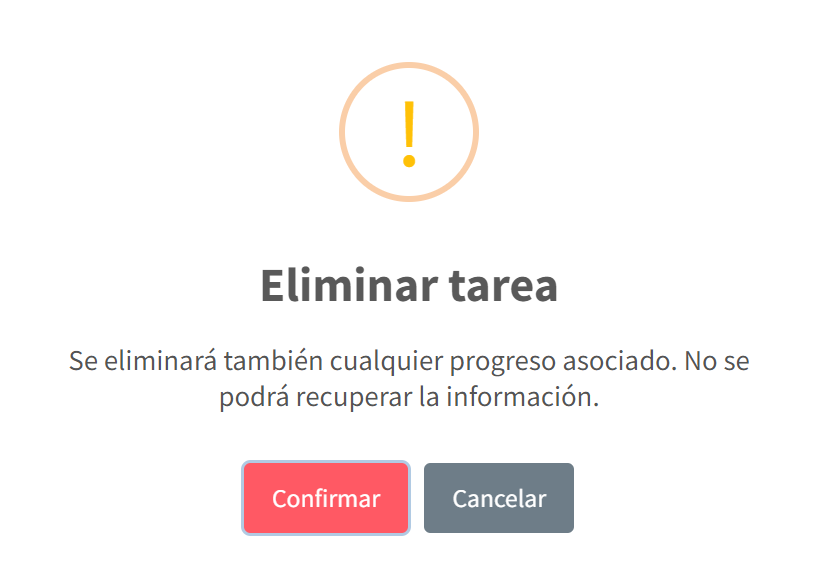
\includegraphics[width=4.16667in,height=\textheight]{./img/manual-user/task-delete.png}

}

\end{figure}

\bookmarksetup{startatroot}

\hypertarget{manual-de-responsable-de-equipo}{%
\chapter{Manual de responsable de
equipo}\label{manual-de-responsable-de-equipo}}

\hypertarget{gestiuxf3n-de-miembros-de-equipo}{%
\section{Gestión de miembros de
equipo}\label{gestiuxf3n-de-miembros-de-equipo}}

El panel de gestión de miembros de equipo permite a una persona
especialmente designada para ello añadir, editar y eliminar usuarios de
los equipos de trabajo. Para acceder al panel de gestión de miembros de
equipo, se debe hacer click en el botón

\includegraphics[width=0.13542in,height=0.17708in]{./img/manual-admin/Tuerca.png}
el cual se encuentra ubicado en la esquina superior derecha de la
pantalla. Al hacer click en ese botón, aparecerá el siguiente menú de
opciones:

\begin{figure}

{\centering \includegraphics[width=5.21875in,height=\textheight]{./img/manual-admin/Menú de opciones.png}

}

\end{figure}

El botón

\includegraphics[width=0.30208in,height=0.23958in]{./img/manual-admin/Botón de gestión de equipos.png}
nos dirige al panel de gestión de miembros del equipo. Una vez que
accedemos al panel, aparecerá un menú de opciones como el siguiente:

\begin{figure}

{\centering \includegraphics{./img/manual-admin/Menú desplegable.png}

}

\end{figure}

Para añadir a un nuevo usuario a algún equipo de trabajo se debe hacer
click en el botón verde ``Agregar'' que se encuentra en la parte
superior del menú de opciones. Nos aparecerá una ventana en la que
podemos seleccionar el usuario específico que queremos incluir dentro de
un equipo, personalizar sus tareas y asignarle un rol específico dentro
del equipo. A continuación se explica el contenido de cada campo.

\includegraphics{./img/manual-admin/Añadir miembro.png}

\textbf{Selecciona usuario}

Este botón presenta una lista de todos los trabajadores que laboran en
una determinada unidad funcional. A partir de esa lista desplegable, se
puede escoger a la persona que se desea incluir dentro de un equipo
específico.

\textbf{Color}

Este botón asignarle a cada usuario un color que permita identificar
rápidamente las tarjetas de tarea que ha creado. De esta manera, cuando
un jefe de equipo visibilice todas las tareas que vienen desarrollando
sus colegas, podrá distinguir a partir del color quién está
desarrollando cada acción.

\textbf{Rol}

Este botón permite asignar un rol específico a cada persona dentro de un
equipo. Existen dos roles que es posible asignar a un determinado
usuario dentro de un equipo: usuario y responsable. El primer tipo de
rol puede añadir, eliminar y avanzar tareas. Por su parte, el segundo
tipo de rol está facultado -además de todas las acciones disponibles
para los usuarios- a visualizar las tareas de todos los miembros de su
equipo y enviar las tareas registradas por cada uno de ellos a la
columna ``Terminado''.

Para modificar la información de algún usuario, es necesario volver al
panel de gestión de de miembros de equipo. Una vez que estamos frente al
menú de opciones, se debe hacer click en el botón amarillo que muestra
el ícono de un lápiz y que se encuentra al lado derecho del nombre del
usuario que se quiere editar. Al hacerlo, aparecerá una ventana como la
siguiente:

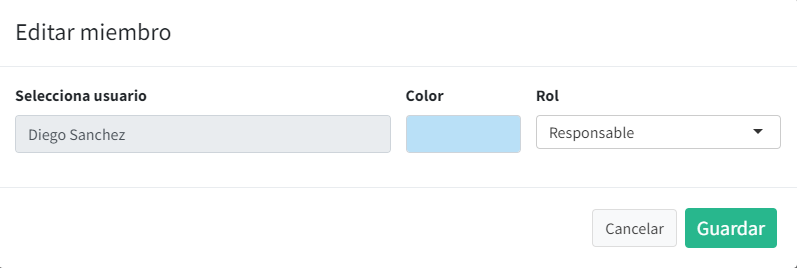
\includegraphics{./img/manual-admin/Editar miembro.png}

Para eliminar a un usuario de un determinado equipo de trabajo, es
necesario volver al panel de gestión de de miembros de equipo. Una vez
que estamos frente al menú de opciones, se debe hacer click en el botón
rojo que muestra el ícono de un tacho de basura y que se encuentra al
lado derecho del nombre del usuario que se quiere eliminar. Al hacerlo
aparecerá una ventana como la siguiente:

\begin{figure}

{\centering 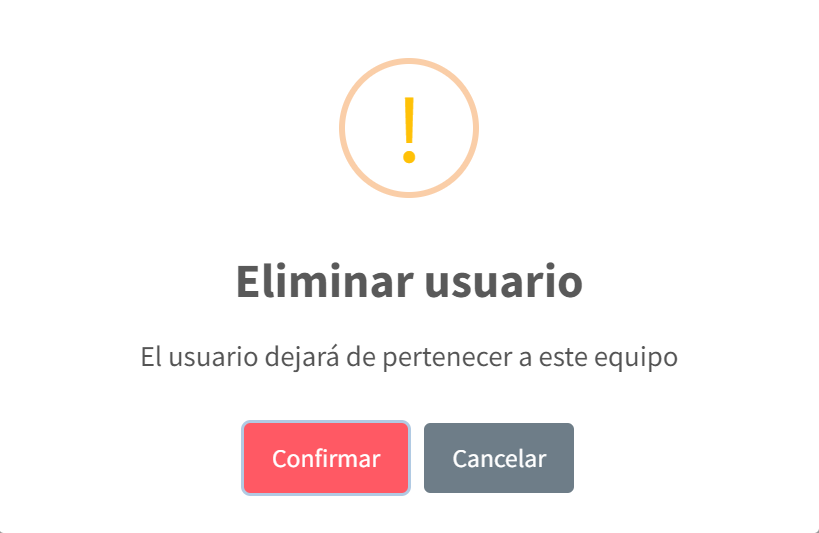
\includegraphics{./img/manual-admin/Eliminar usuario.png}

}

\end{figure}

Para completar la eliminación, solo se debe dar click en el botón
``Confirmar'' y listo.

\hypertarget{gestiuxf3n-de-procesos}{%
\section{Gestión de procesos}\label{gestiuxf3n-de-procesos}}

El panel de gestión de procesos permite a una persona especialmente
designada para ello vincular las tareas implementadas por ciertos
usuarios o equipos específicos al desarrollo de determinados procesos
que se encuentren dentro del marco normativo que regula una determinada
unidad funcional. Para acceder al panel de procesos, se debe hacer click
en el botón

\includegraphics[width=0.13542in,height=0.17708in]{./img/manual-admin/Tuerca.png}
el cual se encuentra ubicado en la esquina superior derecha de la
pantalla. Al hacer click en ese botón, aparecerá el siguiente menú de
opciones:

\begin{figure}

{\centering \includegraphics[width=5.91667in,height=\textheight]{./Menú de opciones 2.png}

}

\end{figure}

El botón

\includegraphics[width=0.29167in,height=0.25in]{./Botón de gestión de procesos.png}
nos dirige al panel de gestión de procesos. Una vez que accedemos al
panel, aparecerá un menú de opciones como el siguiente:

\begin{figure}

{\centering \includegraphics[width=3.65625in,height=\textheight]{./Menú desplegable 2.png}

}

\end{figure}

Para añadir a un nuevo proceso, se debe hacer click en el botón verde
``Agregar'' que se encuentra en la parte superior del menú de opciones.
Nos aparecerá una ventana en la que podemos llenar información del
proceso. A continuación se explica el contenido de cada campo.

\includegraphics{./.pdf}\includegraphics{./Añadir proceso.png}

\textbf{Nombre del proceso}

El título del proceso es la información principal a visualizar. Brinda
una idea general del proceso que determinado usuario o equipo está
cumpliendo al desarrollar sus tareas. Al redactar el título debe
buscarse mantenerlo corto pero lo suficientemente claro para no
confundirlo con otras tareas.

Puede tener como máximo 250 caracteres.

\textbf{Descripción}

La descripción del proceso brinda mayor detalle acerca proceso y al
marco normativo al que está vinculado. Dentro de este campo es posible
explayarse para brindar mayor especificidad al proceso.

Puede tener como máximo 500 caracteres.

Para modificar la información de algún proceso, es necesario volver al
panel de gestión de procesos. Una vez que estamos frente al menú de
opciones, se debe hacer click en el botón amarillo que muestra el ícono
de un lápiz y que se encuentra al lado derecho del nombre del proceso
que se quiere editar. Al hacerlo, aparecerá una ventana como la
siguiente:

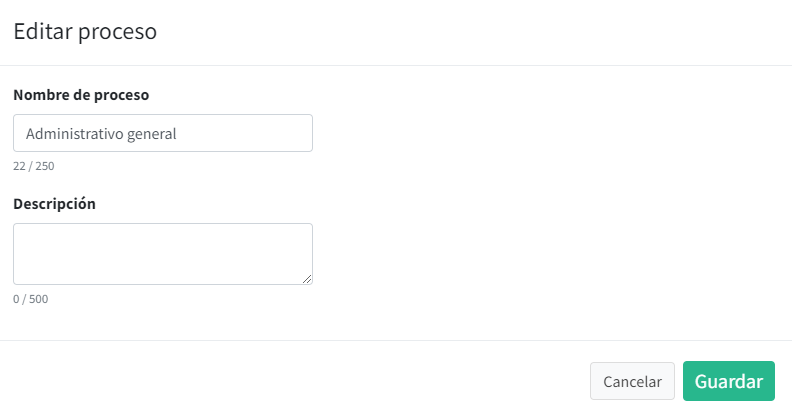
\includegraphics{./Editar proceso.png}

Para eliminar un proceso, es necesario volver al panel de gestión de
gestión. Una vez que estamos frente al menú de opciones, se debe hacer
click en el botón rojo que muestra el ícono de un tacho de basura y que
se encuentra al lado derecho del nombre del proceso que se quiere
eliminar. Al hacerlo aparecerá una ventana como la siguiente:

\begin{figure}

{\centering 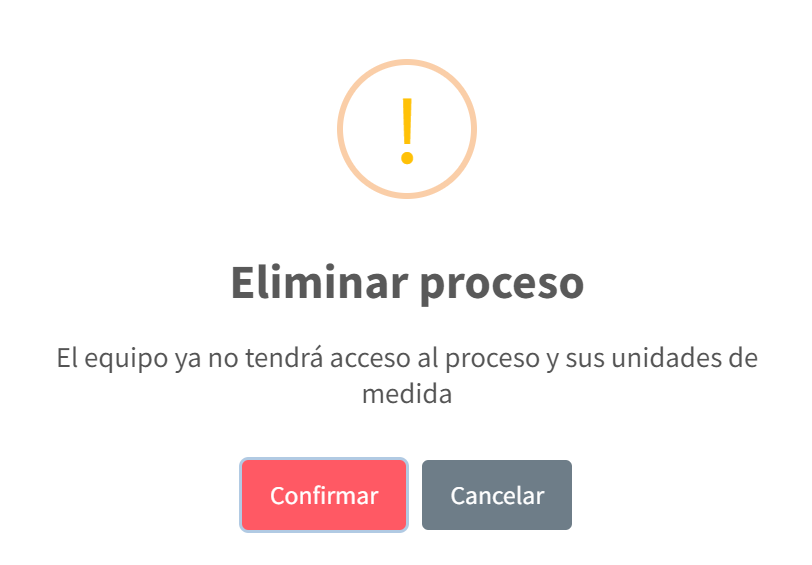
\includegraphics{./Eliminar proceso.png}

}

\end{figure}

\hypertarget{gestiuxf3n-de-unidades-de-medida}{%
\section{Gestión de unidades de
medida}\label{gestiuxf3n-de-unidades-de-medida}}

El panel de gestión de mediciones permite a una persona especialmente
designada para ello vincular los procesos desarrollados por ciertos
usuarios o equipos específicos a productos o evidencias que permitan
medir de la manera más precisa posible los avances de cada usuario o
equipo. Para acceder al panel de gestión de mediciones, se debe hacer
click en el botón

\includegraphics[width=0.13542in,height=0.17708in]{./img/manual-admin/Tuerca.png}
el cual se encuentra ubicado en la esquina superior derecha de la
pantalla. Al hacer click en ese botón, aparecerá el siguiente menú de
opciones:

\begin{figure}

{\centering \includegraphics[width=5.80208in,height=\textheight]{./Menú de opciones 3.png}

}

\end{figure}

El botón

\includegraphics[width=0.28125in,height=0.25in]{./Botón de gestión de mediciones.png}
nos dirige al panel de gestión de mediciones de cada proceso. Una vez
que accedemos al panel, aparecerá un menú de opciones como el siguiente:

\includegraphics{./Menú desplegable 3.png}

Las unidades de medida de tareas son productos y evidencias que permiten
medir el avance en las actividades cotidianas de una determinada unidad
funcional. En ese sentido, sirven como herramienta de monitoreo del
avance de un determinado proceso. Las unidades de medida de tareas
típicas de una unidad funcional son: proyectos de oficios, oficios,
proyectos de memorandos, memorandos, correos o informes. Sin embargo,
debido al tipo de funciones que desempeña, cada proceso desarrollado por
una unidad funcional puede tener unidades de medida distinta. Por su
parte, las unidades de medida de reporte son productos o evidencia que
permiten establecer si es que un proceso se ha completado
satisfactoriamente o no. En ese sentido, sirven como herramienta de
evaluación de un determinado proceso.

Para añadir una nueva unidad de medida de tarea o de reporte, es
necesario primero, hacer click en el menú desplegable titulado
``Seleccionar proceso'' y escoger entre todas las opciones el proceso
específico sobre el cual se va incluir una nueva unidad de medida de
tarea.

Una vez identificado el proceso a partir del cual se va a desarrollar
una unidad de medida, se debe hacer click en el botón verde ``Agregar''
que se encuentra en la parte superior del menú de opciones. Nos
aparecerá una ventana en la que podemos llenar información del proceso.
A continuación se explica el contenido de cada campo.

\begin{figure}

{\centering \includegraphics{./img/manual-admin/Añadir unidad de medida.png}

}

\end{figure}

\textbf{Título de la unidad de medida}

El título de la unidad de medida de tarea o reporte es la información
principal a visualizar. Brinda una idea general del tipo de producto o
evidencia que determinado usuario o equipo va a utilizar para dar cuenta
el avance al desarrollar sus tareas. Al redactar el título debe buscarse
mantenerlo corto pero lo suficientemente claro para no confundirlo con
otras tareas.

Puede tener como máximo 250 caracteres.

\textbf{Descripción}

La descripción de la unidad de medida de tarea o reporte brinda mayor
detalle acerca del producto o evidencia que se está utilizando para dar
cuenta de un determinado proceso. Dentro de este campo es posible
explayarse para brindar mayor especificidad al proceso.

Puede tener como máximo 500 caracteres.

\textbf{Destino}

El destino de la unidad de medida de tarea o reporte permite determinar
si es que la evidencia o producto que se está añadiendo va a servir para
medir una tarea o un reporte, es decir, para definir si es que nos va a
ayudar a mesurar el cumplimiento de una actividad o un proceso.

\textbf{Ícono}

El ícono es una figura estilizada que podemos asignar a una determinada
unidad con el fin de poder identificarla mejor y más fácilmente.

Para modificar la información de alguna unidad de medida de reporte o
tarea, es necesario volver al panel de gestión de mediciones. Una vez
que estamos frente al menú de opciones, se debe hacer click en el botón
amarillo que muestra el ícono de un lápiz y que se encuentra al lado
derecho del nombre de la unidad de medida que se quiere editar. Al
hacerlo, aparecerá una ventana como la siguiente:

\begin{figure}

{\centering 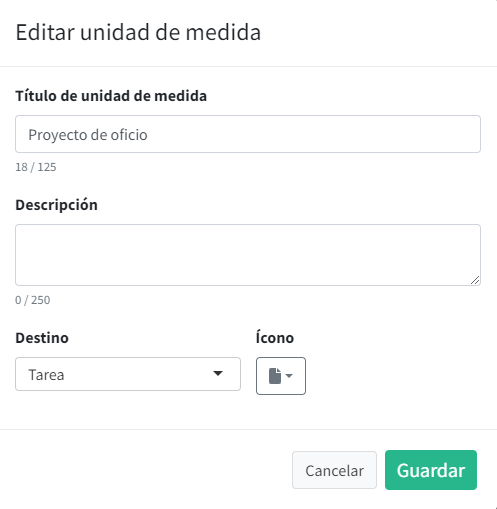
\includegraphics{./img/manual-admin/Editar unidad de medida.png}

}

\end{figure}

Para eliminar una unidad de medida, es necesario volver al panel de
gestión de la medición. Una vez que estamos frente al menú de opciones,
se debe hacer click en el botón rojo que muestra el ícono de un tacho de
basura y que se encuentra al lado derecho del nombre de la unidad de
medida que se quiere eliminar. Al hacerlo aparecerá una ventana como la
siguiente:

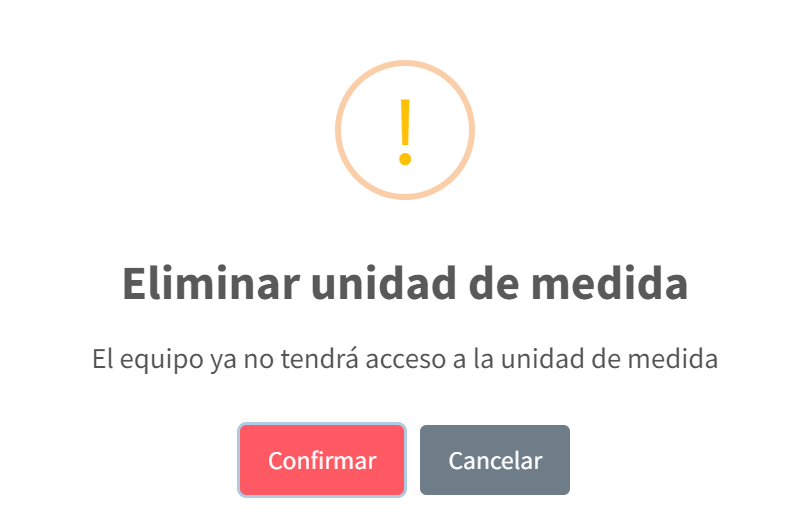
\includegraphics{./img/manual-admin/Eliminar unidad de medida.png}

\hypertarget{descarga-de-reportes}{%
\section{Descarga de reportes}\label{descarga-de-reportes}}

El panel de descarga de reportes permite sistematizar de manera
automatizada en una hoja de cálculo los datos de los avances de las
actividades o procesos -a través de sus respectivas unidades de medida-
que ha venido desarrollando el personal de una determinada unidad
funcional durante un período de tiempo determinado. Para acceder a esta
función debe dirigirse a la parte superior izquierda de la pantalla, más
específicamente, al menú de la columna ``Pendiente''. Se debe hacer
click en el botón \texttt{...} y escoger el item ``Opciones de
descarga''. Nos aparecerá una ventana en la que podemos especificar la
información que queremos descargar. A continuación se explica el
contenido de cada campo.

\includegraphics{./img/manual-admin/Opción de descarga.png}

\textbf{Período de datos}

La opción de período de los datos permite seleccionar el lapso de tiempo
para el cual quiere sistematizar los avances conseguidos en términos de
las actividades o procesos desarrollados por un determinado equipo.

\textbf{Desglosar reporte individual}

La opción de desglosar por reporte individual permite incluir dentro de
la hoja de cálculo la información detallada acerca de cada uno de los
reportes producidos por un equipo dentro del período de tiempo
establecido. De esta manera, la información de cada reporte es asignada
a una columna.

\textbf{Incluir totales}

La opción de incluir totales permite añadir dentro de la hoja de cálculo
una columna que detalle el resultado de la suma de todas las unidades de
medida de los reportes generados por un equipo dentro del período de
tiempo establecido.

\appendix
\addcontentsline{toc}{part}{Appendices}

\hypertarget{sec-ciclo-de-vida}{%
\chapter{Ciclo de vida de una tarea}\label{sec-ciclo-de-vida}}

En el ciclo de vida de una tarea existen las siguientes fases:

\begin{itemize}
\tightlist
\item
  Pendiente
\item
  En proceso
\item
  Pausado
\item
  En revisión
\item
  Observado
\item
  Terminado
\end{itemize}

En este capítulo se explica qué características tiene cada fase. Un
adecuado conocimiento de este ciclo de vida permitirá a los usuarios
generar información valiosa acerca de los tiempos necesarios para el
cumplimiento de sus tareas.

\hypertarget{pendiente}{%
\section{Pendiente}\label{pendiente}}

Indica que la tarea no tiene ningún progreso. Se asigna automáticamente
a tareas recién agregadas. En caso de que el usuario realice progreso en
la tarea, debe avanzar su estado.

No hay un límite respecto al número de tareas que pueden tener este
estado. Un gran acumulado en el número de pendientes podría significar
que se asignan tareas sin tomar en cuenta la carga de trabajo del
usuario. Por el contrario, la ausencia de tareas pendientes podría
significar que no se aprovecha de manera adecuada el recurso humano.

\hypertarget{en-proceso}{%
\section{En proceso}\label{en-proceso}}

Indica que la tarea tiene algún tipo de progreso y el usuario está
activamente trabajando para añadirle más progreso. En esta fase la tarea
necesita aún avances significativos.

Idealmente, cualquier usuario debe tener siempre una tarea en este
estado. Cuando una tarea ``En proceso'' cambia de estado, debe ser
reemplazada por otra.

\hypertarget{pausado}{%
\section{Pausado}\label{pausado}}

Indica que la tarea tiene algún tipo de progreso pero el usuario NO está
activamente trabajando para añadirle más progreso. Debe usarse cuando es
necesario esperar trabajo de otras personas para progresar en la tarea o
cuando una tarea más urgente es añadida, aplazando el cumplimiento de la
actual.

No existe límite respecto al número de tareas que pueden tener este
estado. Sin embargo, si las tareas pasan mucho tiempo en esta fase,
podría significar que la tarea podría haber sido dividida en varias
partes.

\hypertarget{en-revisiuxf3n}{%
\section{En revisión}\label{en-revisiuxf3n}}

Indica que la tarea tiene progreso suficiente como para ser considerada
como terminada. El cambio de fase de la tarea se encuentra a manos del
responsable de equipo.

Si la tarea:

\begin{itemize}
\tightlist
\item
  Está adecuadamente concluida, debe darse por ``Terminada''
\item
  Requiere cambios mínimos -típicamente de forma- para considerarse
  concluida, debe indicarse como ``Observada''
\item
  Requiere cambios sustanciales para considerarse concluida, debe
  indicarse como ``En proceso''.
\end{itemize}

No existe límite respecto al número de tareas que pueden tener este
estado. Sin embargo, si las tareas pasan mucho tiempo en esta fase,
podría significar que el responsable de equipo no está revisando la
finalización de las tareas bajo la lógica de la gestión de la
información.

\hypertarget{observado}{%
\section{Observado}\label{observado}}

Indica que la tarea tiene progreso suficiente como para ser considerada
como terminada pero necesita cambios mínimos antes de darla por
finalizada. Generalmente estos cambios están referidos a correcciones de
formato, ortografía, puntuación y otros relacionados. Una vez finalizada
la corrección debe volver a reportarse como ``En revisión''.

No existe límite respecto al número de tareas que pueden tener este
estado. Si una misma tarea es observada múltiples veces significa que la
retroalimentación por parte del responsable de equipo no está siendo
consistente o que el usuario no está tomando en cuenta la
retroalimentación en su totalidad.

\hypertarget{terminado}{%
\section{Terminado}\label{terminado}}

Indica que la tarea ha sido cumplida satisfactoriamente. Solo se puede
avanzar a esta fase a través de un usuario responsable de equipo.

No existe límite respecto al número de tareas que pueden tener este
estado. El tablero solo muestra las tareas que han sido concluidas en
las últimas dos semanas.



\end{document}
